\documentclass[12pt,a4paper]{article}
\usepackage[spanish]{babel}
\usepackage[utf8]{inputenc}
\usepackage{amsmath}
\usepackage{array}
\usepackage{geometry}
\usepackage{graphicx}
\usepackage{float}
\usepackage{booktabs}
\usepackage{tabularx}
\usepackage[colorlinks=true, linkcolor=blue, citecolor=blue, urlcolor=blue, pdftex]{hyperref}
\geometry{margin=2.5cm}

\title{\textbf{Tercer Trabajo Estadística II} \\[0.5cm]
Correlación y Regresión Múltiple}
\author{
Integrantes: \\ 
1. Juan David Mena Gamboa \\ 
2. Luis Angel Bolaño Lopez \\ 
3. Heyner}
\date{\today}

\begin{document}
\maketitle

\section*{1. Análisis de Correlación}

Utilizando el conjunto de datos de la Gran Encuesta Integrada de Hogares (GEIH) 2024 del DANE, se realizó un análisis de correlación y regresión múltiple. El conjunto de datos incluye las siguientes variables:

\textbf{Variables cuantitativas analizadas:}
\begin{itemize}
    \item \textit{Valor mensual por prácticas o pasantías} (P3087S1): Variable que registra el valor mensual de estas actividades (variable respuesta Y en el modelo de regresión).
    \item \textit{Ahorro por cultivar} (P3094S3): Variable que mide los ingresos netos obtenidos por actividades de cultivo (variable explicativa X$_1$).
    \item \textit{Ahorro por criar animales} (P3095S3): Variable que mide los ingresos netos obtenidos por la cría de animales (variable explicativa X$_2$).
\end{itemize}

\textbf{Variable cualitativa analizada:}
\begin{itemize}
    \item \textit{¿Fue a reuniones familiares durante las últimas 4 semanas?} (P3101): Variable categórica binaria (Sí/No). Esta variable se analiza mediante comparación de medias entre grupos (quienes asistieron vs quienes no asistieron a reuniones familiares) para cada una de las variables cuantitativas, utilizando pruebas de significancia apropiadas (prueba t de Student o prueba de Mann-Whitney según el cumplimiento de supuestos de normalidad).
\end{itemize}

\subsection*{1.1 Pruebas de Significancia de Correlación}

Para cada par de variables se plantearon las hipótesis y se ejecutaron las pruebas de significancia correspondientes utilizando el coeficiente de correlación de Pearson.

\subsubsection*{Relación 1: Valor mensual por prácticas vs Ahorro por cultivar}

\begin{itemize}
    \item \textit{Planteamiento del problema:} Se busca determinar si existe una relación lineal entre el valor mensual por prácticas o pasantías y el ahorro generado por actividades de cultivo en los hogares colombianos.
    \item Hipótesis: \quad $H_0: \rho = 0$ (no hay correlación lineal) \hspace{1cm} $H_1: \rho \neq 0$ (hay correlación lineal)
    \item Nivel de significancia: $\alpha = 0.05$
    \item Estadístico de Prueba: Coeficiente de correlación de Pearson
\end{itemize}

\begin{tabular}{|m{7cm}|m{7cm}|}
\hline
\textbf{Estadístico Empleado} & Correlación de Pearson \\ \hline
\textbf{Fórmula del estadístico} & $t = r\sqrt{\frac{n-2}{1-r^2}}$ \\ \hline
\textbf{Nombre Parámetro} & \textbf{Valor} \\ \hline
Coeficiente de correlación ($r$) & 0.3295 \\ \hline
Estadístico t & 7.7872 \\ \hline
Grados de libertad (df) & 498 \\ \hline
Tamaño de muestra (n) & 500 \\ \hline
Valor-p & $4.00 \times 10^{-14}$ \\ \hline
\end{tabular}

\begin{itemize}
    \item Regla de decisión: Rechazar $H_0$ si p-valor $< 0.05$ o si $|t| > t_{\alpha/2, n-2}$
    \item Decisión: Rechazar $H_0$
    \item Interpretación en el contexto del problema: Con un nivel de significancia de 0.05, la evidencia sugiere que existe una correlación positiva moderada ($r = 0.3295$) entre el valor mensual por prácticas o pasantías y el ahorro generado por actividades de cultivo en los hogares colombianos. Esta relación indica que, en promedio, los hogares que reportan mayores valores mensuales por prácticas o pasantías tienden a tener también mayores ahorros por actividades de cultivo, lo cual podría reflejar que ambos indicadores están relacionados con el nivel de recursos económicos del hogar o con estrategias de diversificación de ingresos. La fuerza de la correlación es moderada ($0.3 \leq |r| < 0.7$), lo que indica una relación lineal de intensidad media entre estas variables.
    \item Comentarios sobre los hallazgos:
    \begin{itemize}
        \item ¿Hay evidencia de correlación?: Sí, existe evidencia estadísticamente significativa de correlación (p-valor $< 0.001$).
        \item ¿En qué dirección?: La correlación es positiva, lo que significa que a medida que aumenta el valor mensual por prácticas, también aumenta el ahorro por cultivar.
        \item ¿Es débil, moderada o fuerte?: La correlación es moderada ($|r| = 0.3295$), lo que indica una relación lineal de intensidad media entre estas variables económicas.
    \end{itemize}
\end{itemize}

\subsubsection*{Relación 2: Valor mensual por prácticas vs Ahorro por criar animales}

\begin{itemize}
    \item \textit{Planteamiento del problema:} Se busca determinar si existe una relación lineal entre el valor mensual por prácticas o pasantías y el ahorro generado por la cría de animales en los hogares colombianos.
    \item Hipótesis: \quad $H_0: \rho = 0$ (no hay correlación lineal) \hspace{1cm} $H_1: \rho \neq 0$ (hay correlación lineal)
    \item Nivel de significancia: $\alpha = 0.05$
    \item Estadístico de Prueba: Coeficiente de correlación de Pearson
\end{itemize}

\begin{tabular}{|m{7cm}|m{7cm}|}
\hline
\textbf{Estadístico Empleado} & Correlación de Pearson \\ \hline
\textbf{Fórmula del estadístico} & $t = r\sqrt{\frac{n-2}{1-r^2}}$ \\ \hline
\textbf{Nombre Parámetro} & \textbf{Valor} \\ \hline
Coeficiente de correlación ($r$) & 0.2226 \\ \hline
Estadístico t & 5.0962 \\ \hline
Grados de libertad (df) & 498 \\ \hline
Tamaño de muestra (n) & 500 \\ \hline
Valor-p & $4.93 \times 10^{-7}$ \\ \hline
\end{tabular}

\begin{itemize}
    \item Regla de decisión: Rechazar $H_0$ si p-valor $< 0.05$ o si $|t| > t_{\alpha/2, n-2}$
    \item Decisión: Rechazar $H_0$
    \item Interpretación en el contexto del problema: Con un nivel de significancia de 0.05, la evidencia sugiere que existe una correlación positiva débil ($r = 0.2226$) entre el valor mensual por prácticas o pasantías y el ahorro generado por la cría de animales en los hogares colombianos. Esta relación indica que, en promedio, los hogares que reportan mayores valores mensuales por prácticas o pasantías tienden a tener también mayores ahorros por la cría de animales, aunque esta asociación es menos fuerte que la observada con el ahorro por cultivar. Esta relación podría reflejar que ambas actividades económicas están relacionadas con el nivel de recursos del hogar, pero la cría de animales podría estar más asociada con contextos rurales o periurbanos específicos, mientras que las prácticas tienen una distribución más amplia. La fuerza de la correlación es débil ($0.1 \leq |r| < 0.3$), lo que indica una relación lineal de baja intensidad entre estas variables.
    \item Comentarios sobre los hallazgos:
    \begin{itemize}
        \item ¿Hay evidencia de correlación?: Sí, existe evidencia estadísticamente significativa de correlación (p-valor $< 0.001$).
        \item ¿En qué dirección?: La correlación es positiva, lo que significa que a medida que aumenta el valor mensual por prácticas, también aumenta el ahorro por criar animales.
        \item ¿Es débil, moderada o fuerte?: La correlación es débil ($|r| = 0.2226$), lo que indica una relación lineal de baja intensidad entre estas variables económicas.
    \end{itemize}
\end{itemize}

\subsubsection*{Relación 3: Ahorro por cultivar vs Ahorro por criar animales}

\begin{itemize}
    \item \textit{Planteamiento del problema:} Se busca determinar si existe una relación lineal entre el ahorro generado por actividades de cultivo y el ahorro generado por la cría de animales en los hogares colombianos.
    \item Hipótesis: \quad $H_0: \rho = 0$ (no hay correlación lineal) \hspace{1cm} $H_1: \rho \neq 0$ (hay correlación lineal)
    \item Nivel de significancia: $\alpha = 0.05$
    \item Estadístico de Prueba: Coeficiente de correlación de Pearson
\end{itemize}

\begin{tabular}{|m{7cm}|m{7cm}|}
\hline
\textbf{Estadístico Empleado} & Correlación de Pearson \\ \hline
\textbf{Fórmula del estadístico} & $t = r\sqrt{\frac{n-2}{1-r^2}}$ \\ \hline
\textbf{Nombre Parámetro} & \textbf{Valor} \\ \hline
Coeficiente de correlación ($r$) & 0.1344 \\ \hline
Estadístico t & 3.0257 \\ \hline
Grados de libertad (df) & 498 \\ \hline
Tamaño de muestra (n) & 500 \\ \hline
Valor-p & $2.61 \times 10^{-3}$ \\ \hline
\end{tabular}

\begin{itemize}
    \item Regla de decisión: Rechazar $H_0$ si p-valor $< 0.05$ o si $|t| > t_{\alpha/2, n-2}$
    \item Decisión: Rechazar $H_0$
    \item Interpretación en el contexto del problema: Con un nivel de significancia de 0.05, la evidencia sugiere que existe una correlación positiva débil ($r = 0.1344$) entre el ahorro generado por actividades de cultivo y el ahorro generado por la cría de animales en los hogares colombianos. Esta relación indica que, en promedio, los hogares que reportan mayores ahorros por cultivar tienden a tener también mayores ahorros por criar animales, aunque esta asociación es muy débil. Esta relación podría reflejar que ambos tipos de actividades agropecuarias están presentes en hogares rurales que diversifican sus fuentes de ingresos, pero la baja correlación sugiere que estos son estrategias económicas que pueden funcionar de manera relativamente independiente. La fuerza de la correlación es débil ($0.1 \leq |r| < 0.3$), lo que indica una relación lineal de baja intensidad entre estas variables. La baja correlación entre estas dos variables explicativas es favorable para el modelo de regresión múltiple, ya que reduce el riesgo de multicolinealidad.
    \item Comentarios sobre los hallazgos:
    \begin{itemize}
        \item ¿Hay evidencia de correlación?: Sí, existe evidencia estadísticamente significativa de correlación (p-valor = 0.0026).
        \item ¿En qué dirección?: La correlación es positiva, lo que significa que a medida que aumenta el ahorro por cultivar, también aumenta el ahorro por criar animales.
        \item ¿Es débil, moderada o fuerte?: La correlación es débil ($|r| = 0.1344$), lo que indica una relación lineal de baja intensidad entre estas variables económicas. Esta baja correlación es beneficiosa para el modelo de regresión múltiple, ya que reduce el riesgo de problemas de multicolinealidad entre las variables explicativas.
    \end{itemize}
\end{itemize}

\subsection*{1.2 Matriz de Correlación}

A continuación se presentan las representaciones gráficas de las correlaciones entre las variables analizadas. La Figura \ref{fig:correlograma} muestra la matriz de correlación de Pearson entre las tres variables analizadas.

\begin{figure}[H]
    \centering
    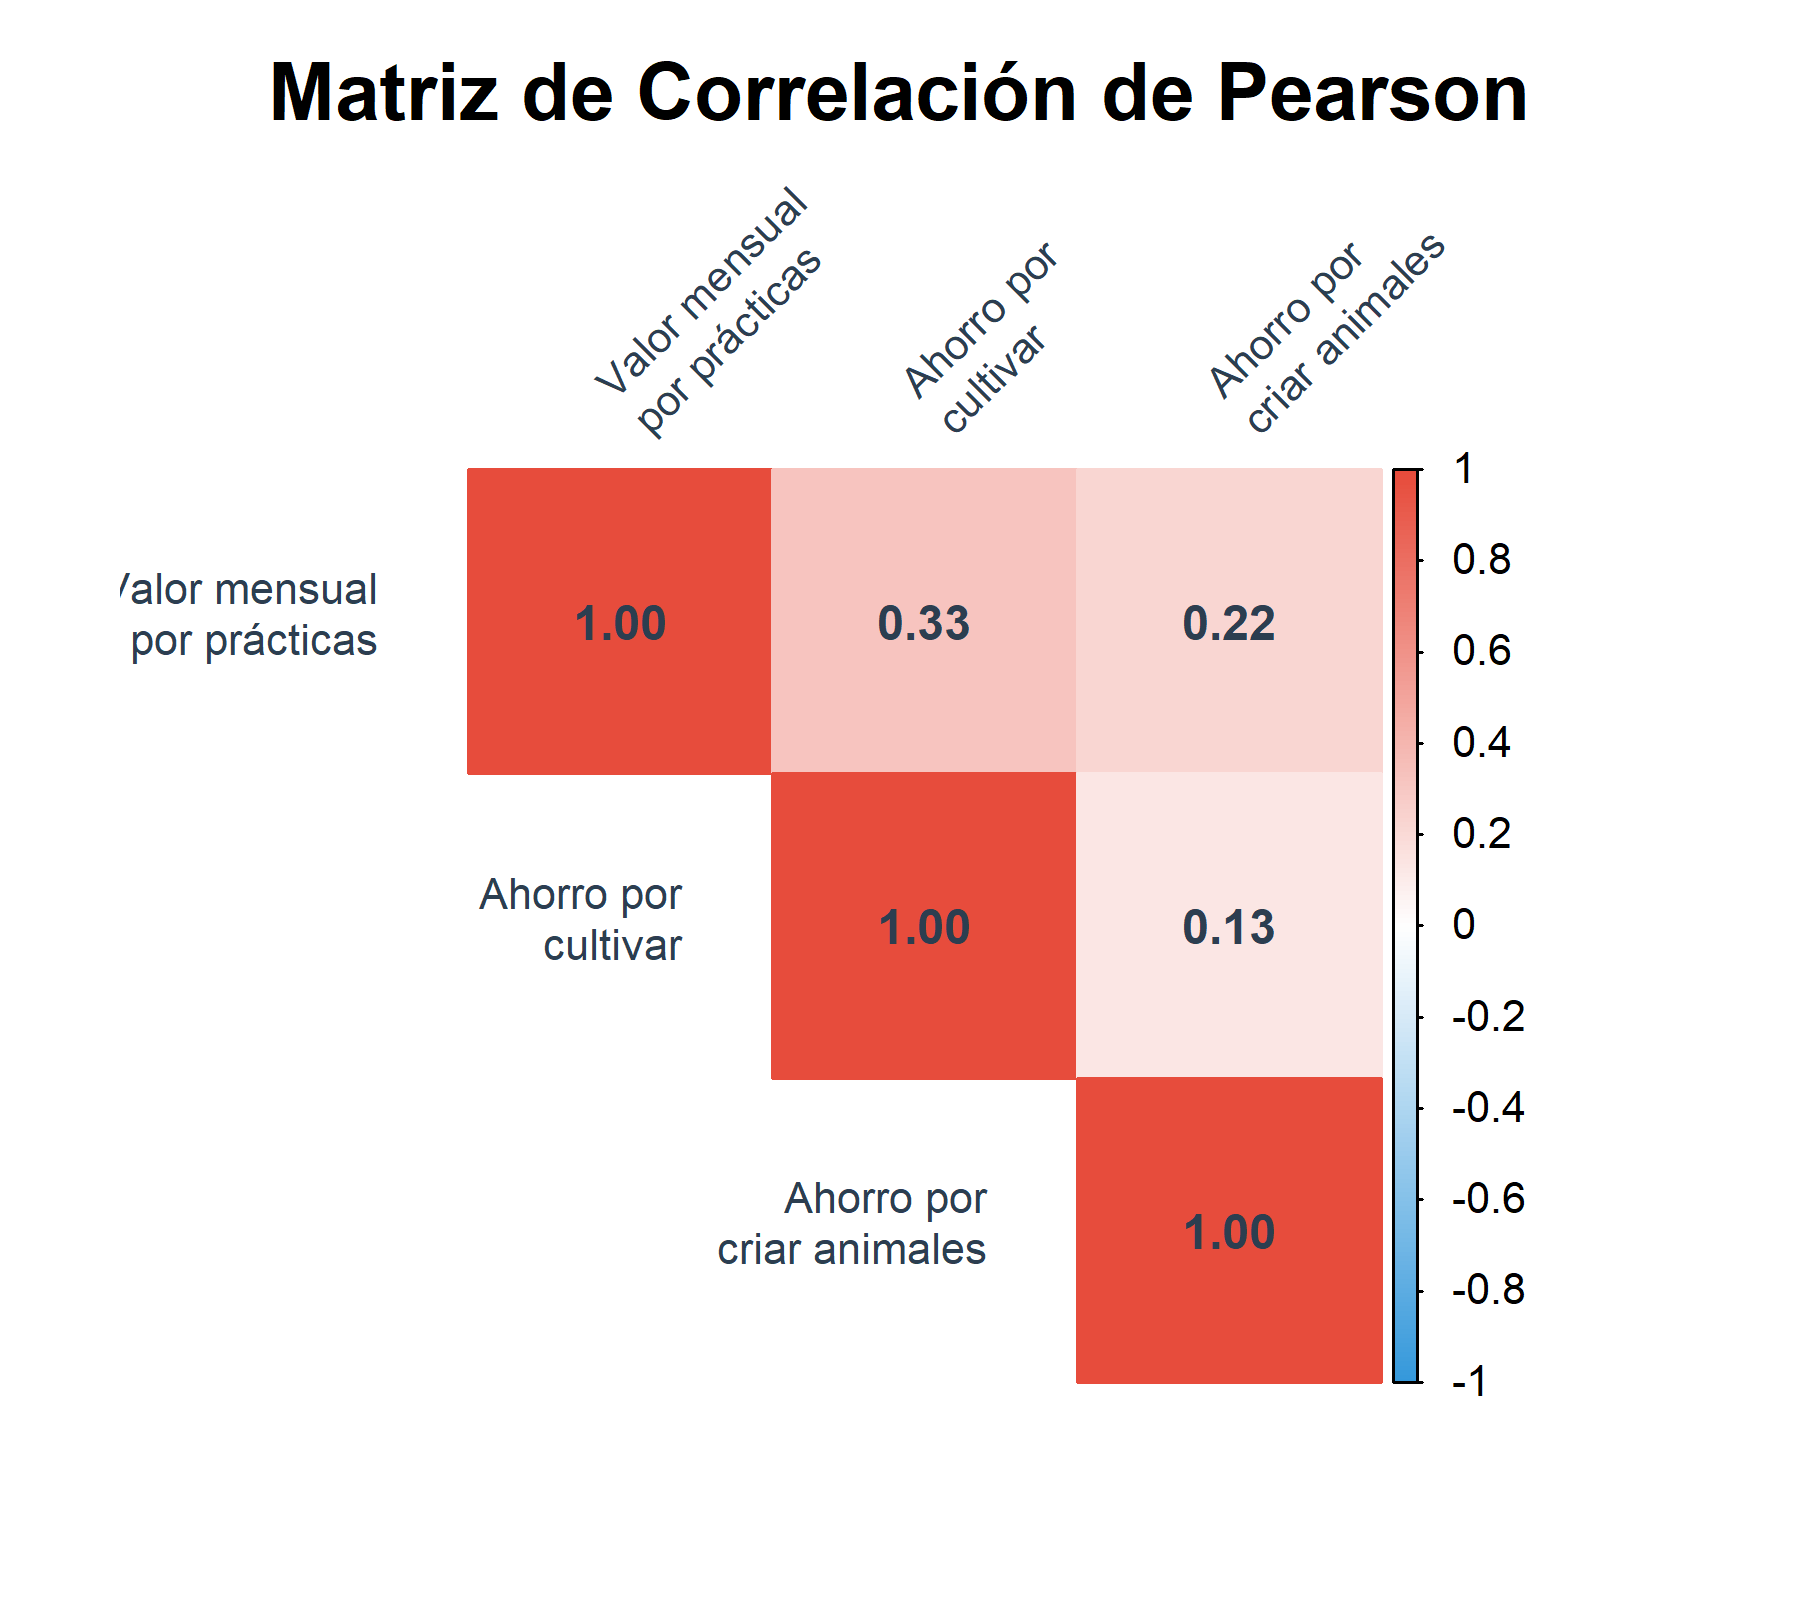
\includegraphics[width=0.8\textwidth]{../Taller 3/plots/correlograma.png}
    \caption{Matriz de Correlación de Pearson}
    \label{fig:correlograma}
\end{figure}

En la Figura \ref{fig:correlograma} se observa que todos los coeficientes de correlación son positivos, lo cual indica relaciones directas entre las variables. Los colores más intensos (rojos más oscuros) representan correlaciones más fuertes. La correlación más fuerte es la que existe entre el valor mensual por prácticas y el ahorro por cultivar (r = 0.330), seguida por la correlación entre el valor mensual por prácticas y el ahorro por criar animales (r = 0.223). La correlación más débil es la que existe entre las dos variables explicativas, ahorro por cultivar y ahorro por criar animales (r = 0.134), lo cual es favorable para evitar problemas de multicolinealidad en el modelo de regresión.

La Figura \ref{fig:matriz_dispersion} presenta la matriz de dispersión que incluye diagramas de dispersión entre pares de variables y las distribuciones marginales de cada variable en la diagonal.

\begin{figure}[H]
    \centering
    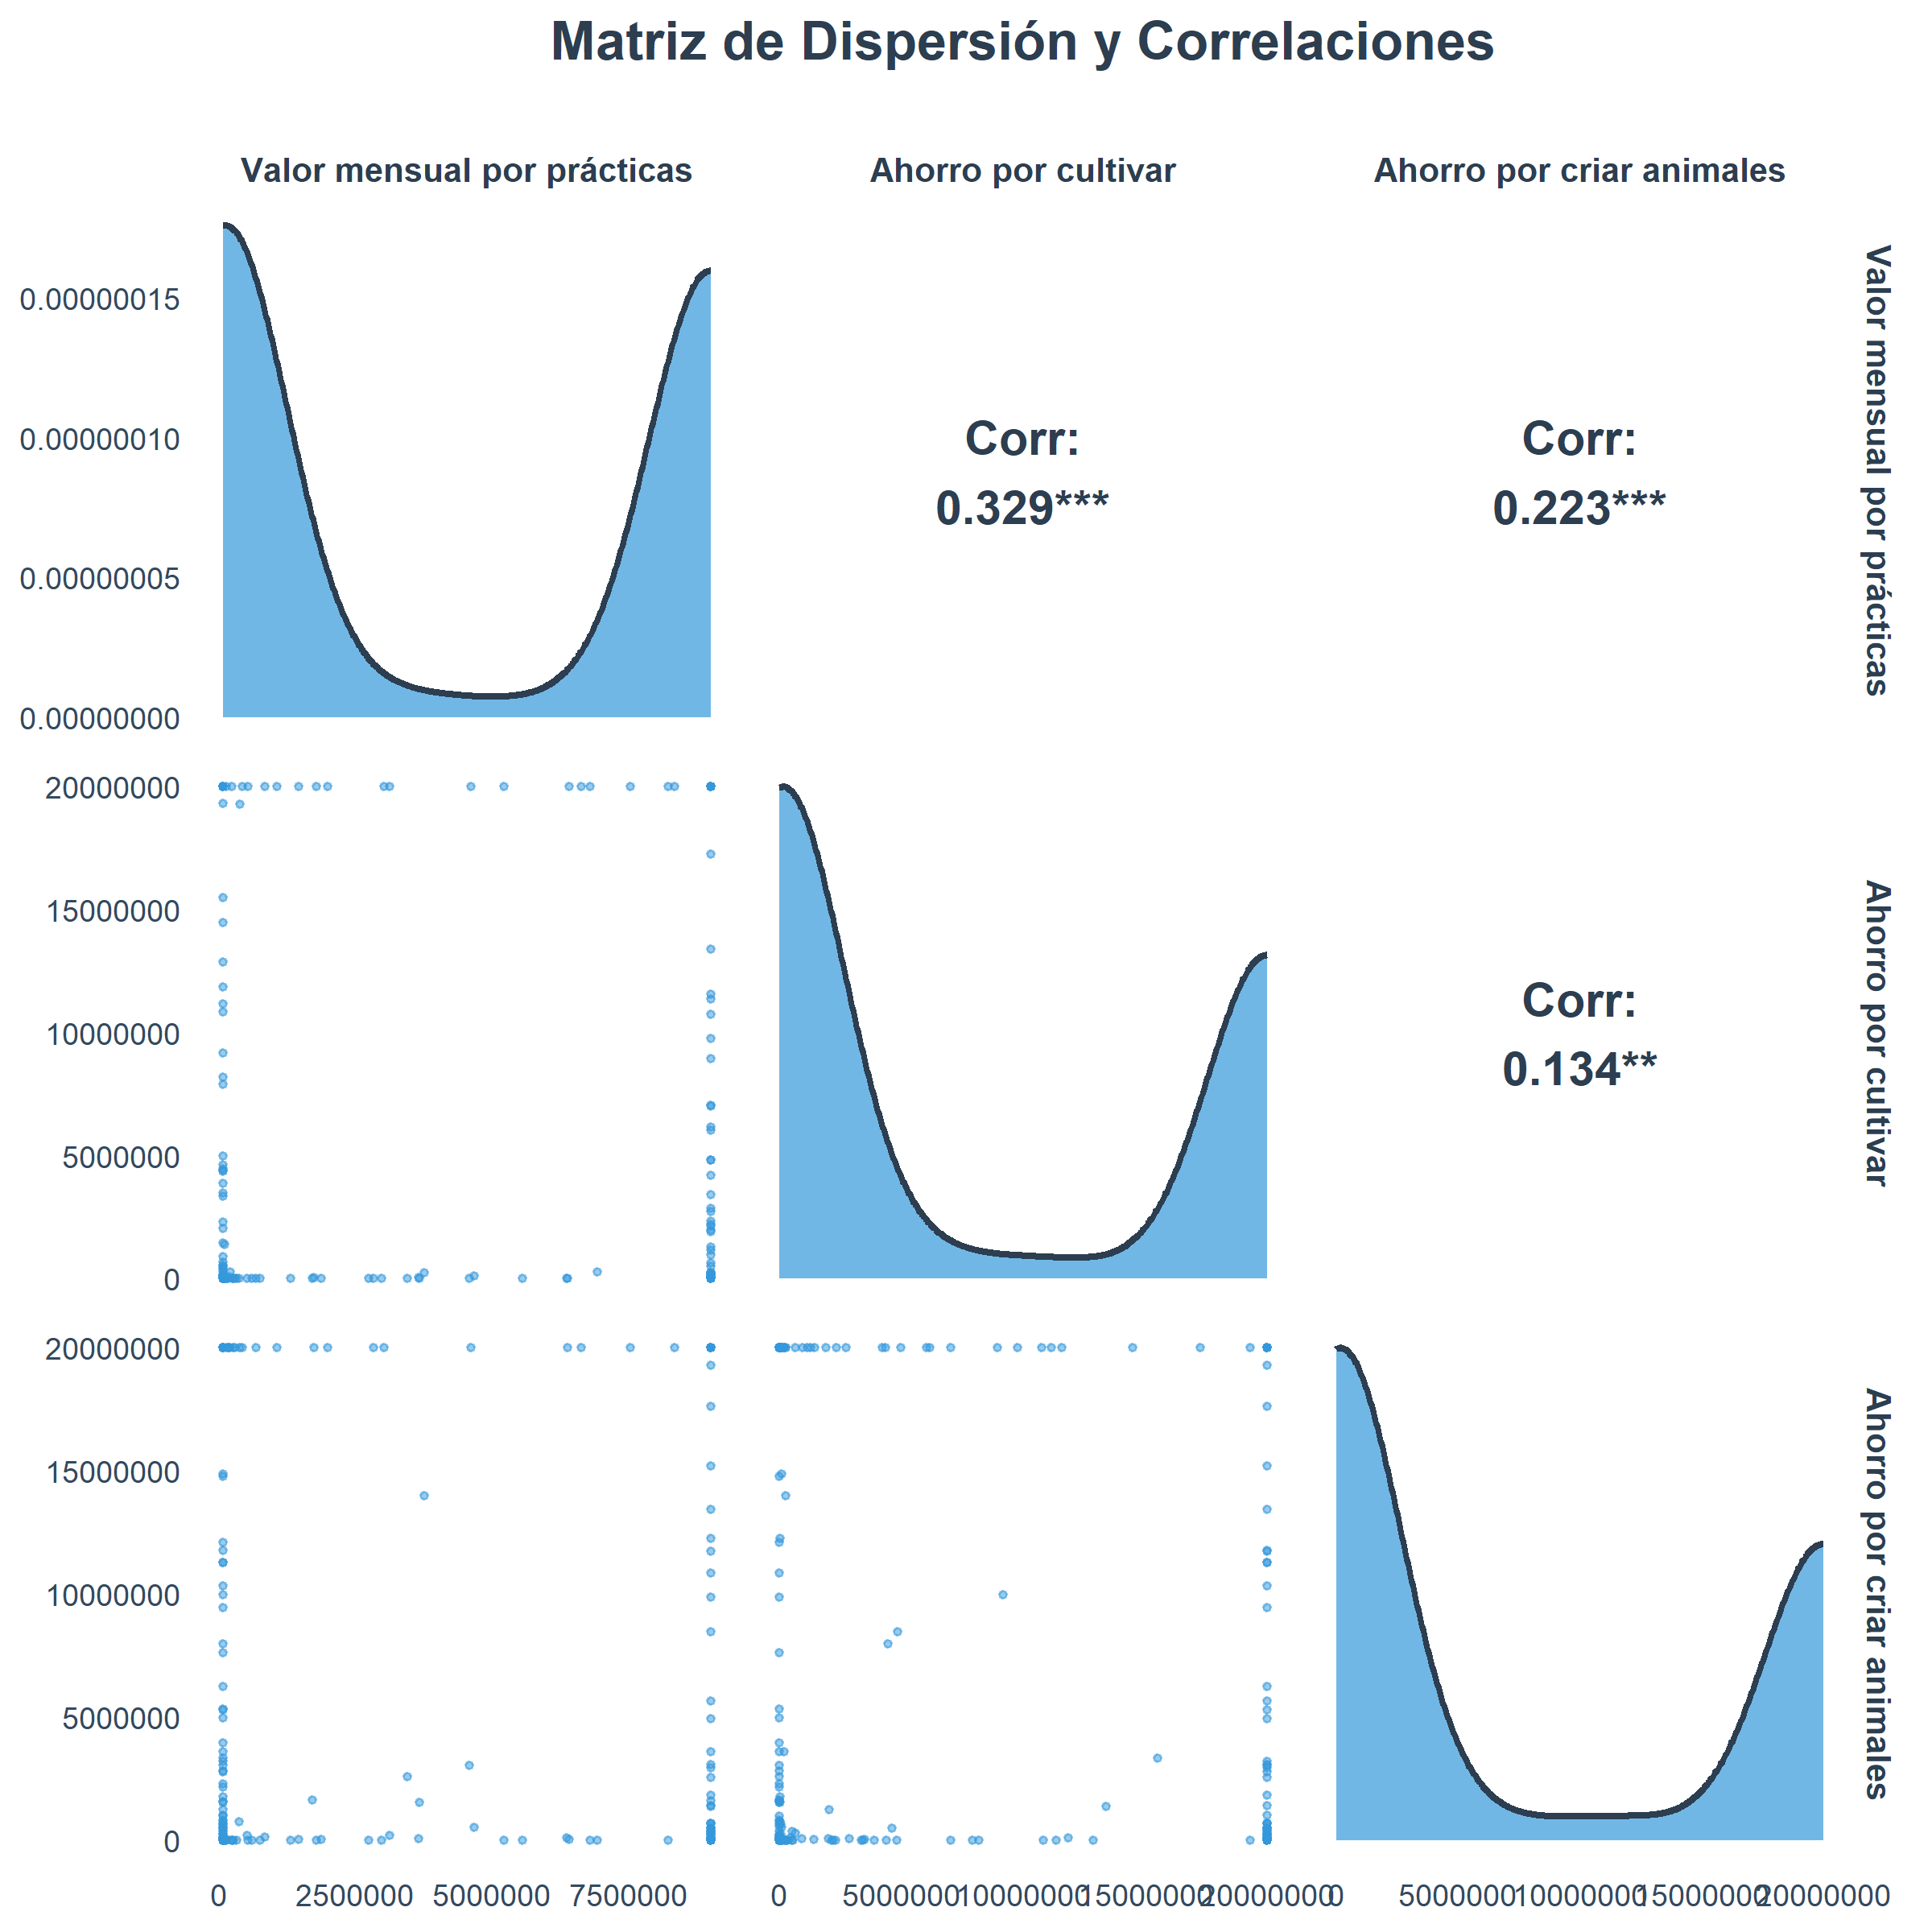
\includegraphics[width=1.0\textwidth]{../Taller 3/plots/matriz_dispersion.png}
    \caption{Matriz de Dispersión y Correlaciones}
    \label{fig:matriz_dispersion}
\end{figure}

En la Figura \ref{fig:matriz_dispersion} se observan los diagramas de dispersión entre cada par de variables, los cuales muestran tendencias positivas en todas las relaciones, confirmando las correlaciones positivas encontradas. En la diagonal se presentan las distribuciones de frecuencia de cada variable, las cuales muestran distribuciones sesgadas hacia la derecha, característica común en variables económicas que representan valores monetarios. Este patrón indica que la mayoría de los hogares tienen valores relativamente bajos en estas variables, mientras que algunos hogares presentan valores considerablemente más altos, lo cual es consistente con la distribución típica de ingresos y ahorros en poblaciones económicas.

\subsection*{1.3 Análisis Comparativo con Variable Cualitativa: Reuniones Familiares}

Para analizar la asociación entre la variable cualitativa P3101 (¿Fue a reuniones familiares durante las últimas 4 semanas?) y las variables cuantitativas, se realizó un análisis comparativo de medias entre los dos grupos (Sí vs No) para cada variable cuantitativa. Dado que la correlación de Pearson requiere variables continuas, se utilizaron pruebas de comparación de medias (prueba t de Student o prueba de Mann-Whitney según el cumplimiento de supuestos de normalidad).

\subsubsection*{Relación 4: Valor mensual por prácticas vs Reuniones familiares}

\begin{itemize}
    \item \textit{Planteamiento del problema:} Se busca determinar si existe una diferencia significativa en el valor mensual por prácticas o pasantías entre las personas que asistieron a reuniones familiares y las que no asistieron.
    \item Hipótesis: \quad $H_0: \mu_{\text{Sí}} = \mu_{\text{No}}$ (no hay diferencia entre grupos) \hspace{1cm} $H_1: \mu_{\text{Sí}} \neq \mu_{\text{No}}$ (hay diferencia entre grupos)
    \item Nivel de significancia: $\alpha = 0.05$
    \item Estadístico de Prueba: Prueba de Mann-Whitney (U de Wilcoxon)
\end{itemize}

\begin{tabular}{|m{7cm}|m{7cm}|}
\hline
\textbf{Estadístico Empleado} & Prueba de Mann-Whitney (U de Wilcoxon) \\ \hline
\textbf{Nombre Parámetro} & \textbf{Valor} \\ \hline
Grupo 'Sí' (asistió a reuniones familiares): n & 4 \\ \hline
Grupo 'Sí': Media & 986,250 \\ \hline
Grupo 'No' (no asistió a reuniones familiares): n & 332 \\ \hline
Grupo 'No': Media & 998,858.4 \\ \hline
Diferencia de medias (Sí - No) & -12,608.43 \\ \hline
Estadístico U (Mann-Whitney) & 651 \\ \hline
Valor-p & 0.948 \\ \hline
\end{tabular}

\begin{itemize}
    \item Regla de decisión: Rechazar $H_0$ si p-valor $< 0.05$
    \item Decisión: No rechazar $H_0$
    \item Interpretación en el contexto del problema: Con un nivel de significancia de 0.05, no hay evidencia estadísticamente significativa de diferencia en el valor mensual por prácticas o pasantías entre las personas que asistieron a reuniones familiares (media = 986,250) y las que no asistieron (media = 998,858.4). La diferencia observada (-12,608.43) no es estadísticamente significativa (p-valor = 0.948). Esto indica que la asistencia a reuniones familiares no está asociada con diferencias en el valor mensual por prácticas o pasantías.
    \item Comentarios sobre los hallazgos:
    \begin{itemize}
        \item ¿Hay evidencia de asociación?: No, no hay evidencia estadísticamente significativa de asociación (p-valor = 0.948 $> 0.05$).
        \item ¿En qué dirección?: Sin diferencia significativa (la diferencia observada no es estadísticamente significativa).
        \item ¿Es débil, moderada o fuerte?: Sin efecto (no hay diferencia significativa entre grupos).
    \end{itemize}
\end{itemize}

\subsubsection*{Relación 5: Ahorro por cultivar vs Reuniones familiares}

\begin{itemize}
    \item \textit{Planteamiento del problema:} Se busca determinar si existe una diferencia significativa en el ahorro por cultivar entre las personas que asistieron a reuniones familiares y las que no asistieron.
    \item Hipótesis: \quad $H_0: \mu_{\text{Sí}} = \mu_{\text{No}}$ (no hay diferencia entre grupos) \hspace{1cm} $H_1: \mu_{\text{Sí}} \neq \mu_{\text{No}}$ (hay diferencia entre grupos)
    \item Nivel de significancia: $\alpha = 0.05$
    \item Estadístico de Prueba: Prueba de Mann-Whitney (U de Wilcoxon)
\end{itemize}

\begin{tabular}{|m{7cm}|m{7cm}|}
\hline
\textbf{Estadístico Empleado} & Prueba de Mann-Whitney (U de Wilcoxon) \\ \hline
\textbf{Nombre Parámetro} & \textbf{Valor} \\ \hline
Grupo 'Sí' (asistió a reuniones familiares): n & 355 \\ \hline
Grupo 'Sí': Media & 107,085.9 \\ \hline
Grupo 'No' (no asistió a reuniones familiares): n & 2,537 \\ \hline
Grupo 'No': Media & 129,715.4 \\ \hline
Diferencia de medias (Sí - No) & -22,629.47 \\ \hline
Estadístico U (Mann-Whitney) & 426,349 \\ \hline
Valor-p & 0.103 \\ \hline
\end{tabular}

\begin{itemize}
    \item Regla de decisión: Rechazar $H_0$ si p-valor $< 0.05$
    \item Decisión: No rechazar $H_0$
    \item Interpretación en el contexto del problema: Con un nivel de significancia de 0.05, no hay evidencia estadísticamente significativa de diferencia en el ahorro por cultivar entre las personas que asistieron a reuniones familiares (media = 107,085.9) y las que no asistieron (media = 129,715.4). Aunque se observa una diferencia numérica (-22,629.47) donde el grupo que no asistió tiene un mayor ahorro promedio, esta diferencia no es estadísticamente significativa (p-valor = 0.103). Esto indica que la asistencia a reuniones familiares no está asociada con diferencias significativas en el ahorro por cultivar.
    \item Comentarios sobre los hallazgos:
    \begin{itemize}
        \item ¿Hay evidencia de asociación?: No, no hay evidencia estadísticamente significativa de asociación (p-valor = 0.103 $> 0.05$).
        \item ¿En qué dirección?: Sin diferencia significativa (aunque hay una diferencia numérica donde el grupo 'No' tiene mayor media, esta diferencia no es estadísticamente significativa).
        \item ¿Es débil, moderada o fuerte?: Sin efecto (no hay diferencia significativa entre grupos).
    \end{itemize}
\end{itemize}

\subsubsection*{Relación 6: Ahorro por criar animales vs Reuniones familiares}

\begin{itemize}
    \item \textit{Planteamiento del problema:} Se busca determinar si existe una diferencia significativa en el ahorro por criar animales entre las personas que asistieron a reuniones familiares y las que no asistieron.
    \item Hipótesis: \quad $H_0: \mu_{\text{Sí}} = \mu_{\text{No}}$ (no hay diferencia entre grupos) \hspace{1cm} $H_1: \mu_{\text{Sí}} \neq \mu_{\text{No}}$ (hay diferencia entre grupos)
    \item Nivel de significancia: $\alpha = 0.05$
    \item Estadístico de Prueba: Prueba de Mann-Whitney (U de Wilcoxon)
\end{itemize}

\begin{tabular}{|m{7cm}|m{7cm}|}
\hline
\textbf{Estadístico Empleado} & Prueba de Mann-Whitney (U de Wilcoxon) \\ \hline
\textbf{Nombre Parámetro} & \textbf{Valor} \\ \hline
Grupo 'Sí' (asistió a reuniones familiares): n & 420 \\ \hline
Grupo 'Sí': Media & 116,109.5 \\ \hline
Grupo 'No' (no asistió a reuniones familiares): n & 3,660 \\ \hline
Grupo 'No': Media & 164,447.3 \\ \hline
Diferencia de medias (Sí - No) & -48,337.8 \\ \hline
Estadístico U (Mann-Whitney) & 726,961 \\ \hline
Valor-p & 0.068 \\ \hline
\end{tabular}

\begin{itemize}
    \item Regla de decisión: Rechazar $H_0$ si p-valor $< 0.05$
    \item Decisión: No rechazar $H_0$
    \item Interpretación en el contexto del problema: Con un nivel de significancia de 0.05, no hay evidencia estadísticamente significativa de diferencia en el ahorro por criar animales entre las personas que asistieron a reuniones familiares (media = 116,109.5) y las que no asistieron (media = 164,447.3). Aunque se observa una diferencia numérica considerable (-48,337.8) donde el grupo que no asistió tiene un mayor ahorro promedio, esta diferencia no alcanza significancia estadística (p-valor = 0.068, ligeramente por encima del umbral de 0.05). Esto indica que la asistencia a reuniones familiares no está asociada con diferencias estadísticamente significativas en el ahorro por criar animales, aunque existe una tendencia numérica que sugiere que quienes no asistieron a reuniones familiares podrían tener mayores ahorros por criar animales.
    \item Comentarios sobre los hallazgos:
    \begin{itemize}
        \item ¿Hay evidencia de asociación?: No, no hay evidencia estadísticamente significativa de asociación (p-valor = 0.068 $> 0.05$), aunque el p-valor está cerca del umbral de significancia.
        \item ¿En qué dirección?: Sin diferencia significativa (aunque hay una diferencia numérica considerable donde el grupo 'No' tiene mayor media, esta diferencia no alcanza significancia estadística al nivel $\alpha = 0.05$).
        \item ¿Es débil, moderada o fuerte?: Sin efecto estadísticamente significativo (aunque hay una tendencia numérica que podría ser de interés para análisis posteriores con mayor poder estadístico o niveles de significancia menos estrictos).
    \end{itemize}
\end{itemize}

La Figura \ref{fig:comparativo_p3101} presenta los diagramas de caja (boxplots) comparativos para cada variable cuantitativa según el grupo de reuniones familiares.

\begin{figure}[H]
    \centering
    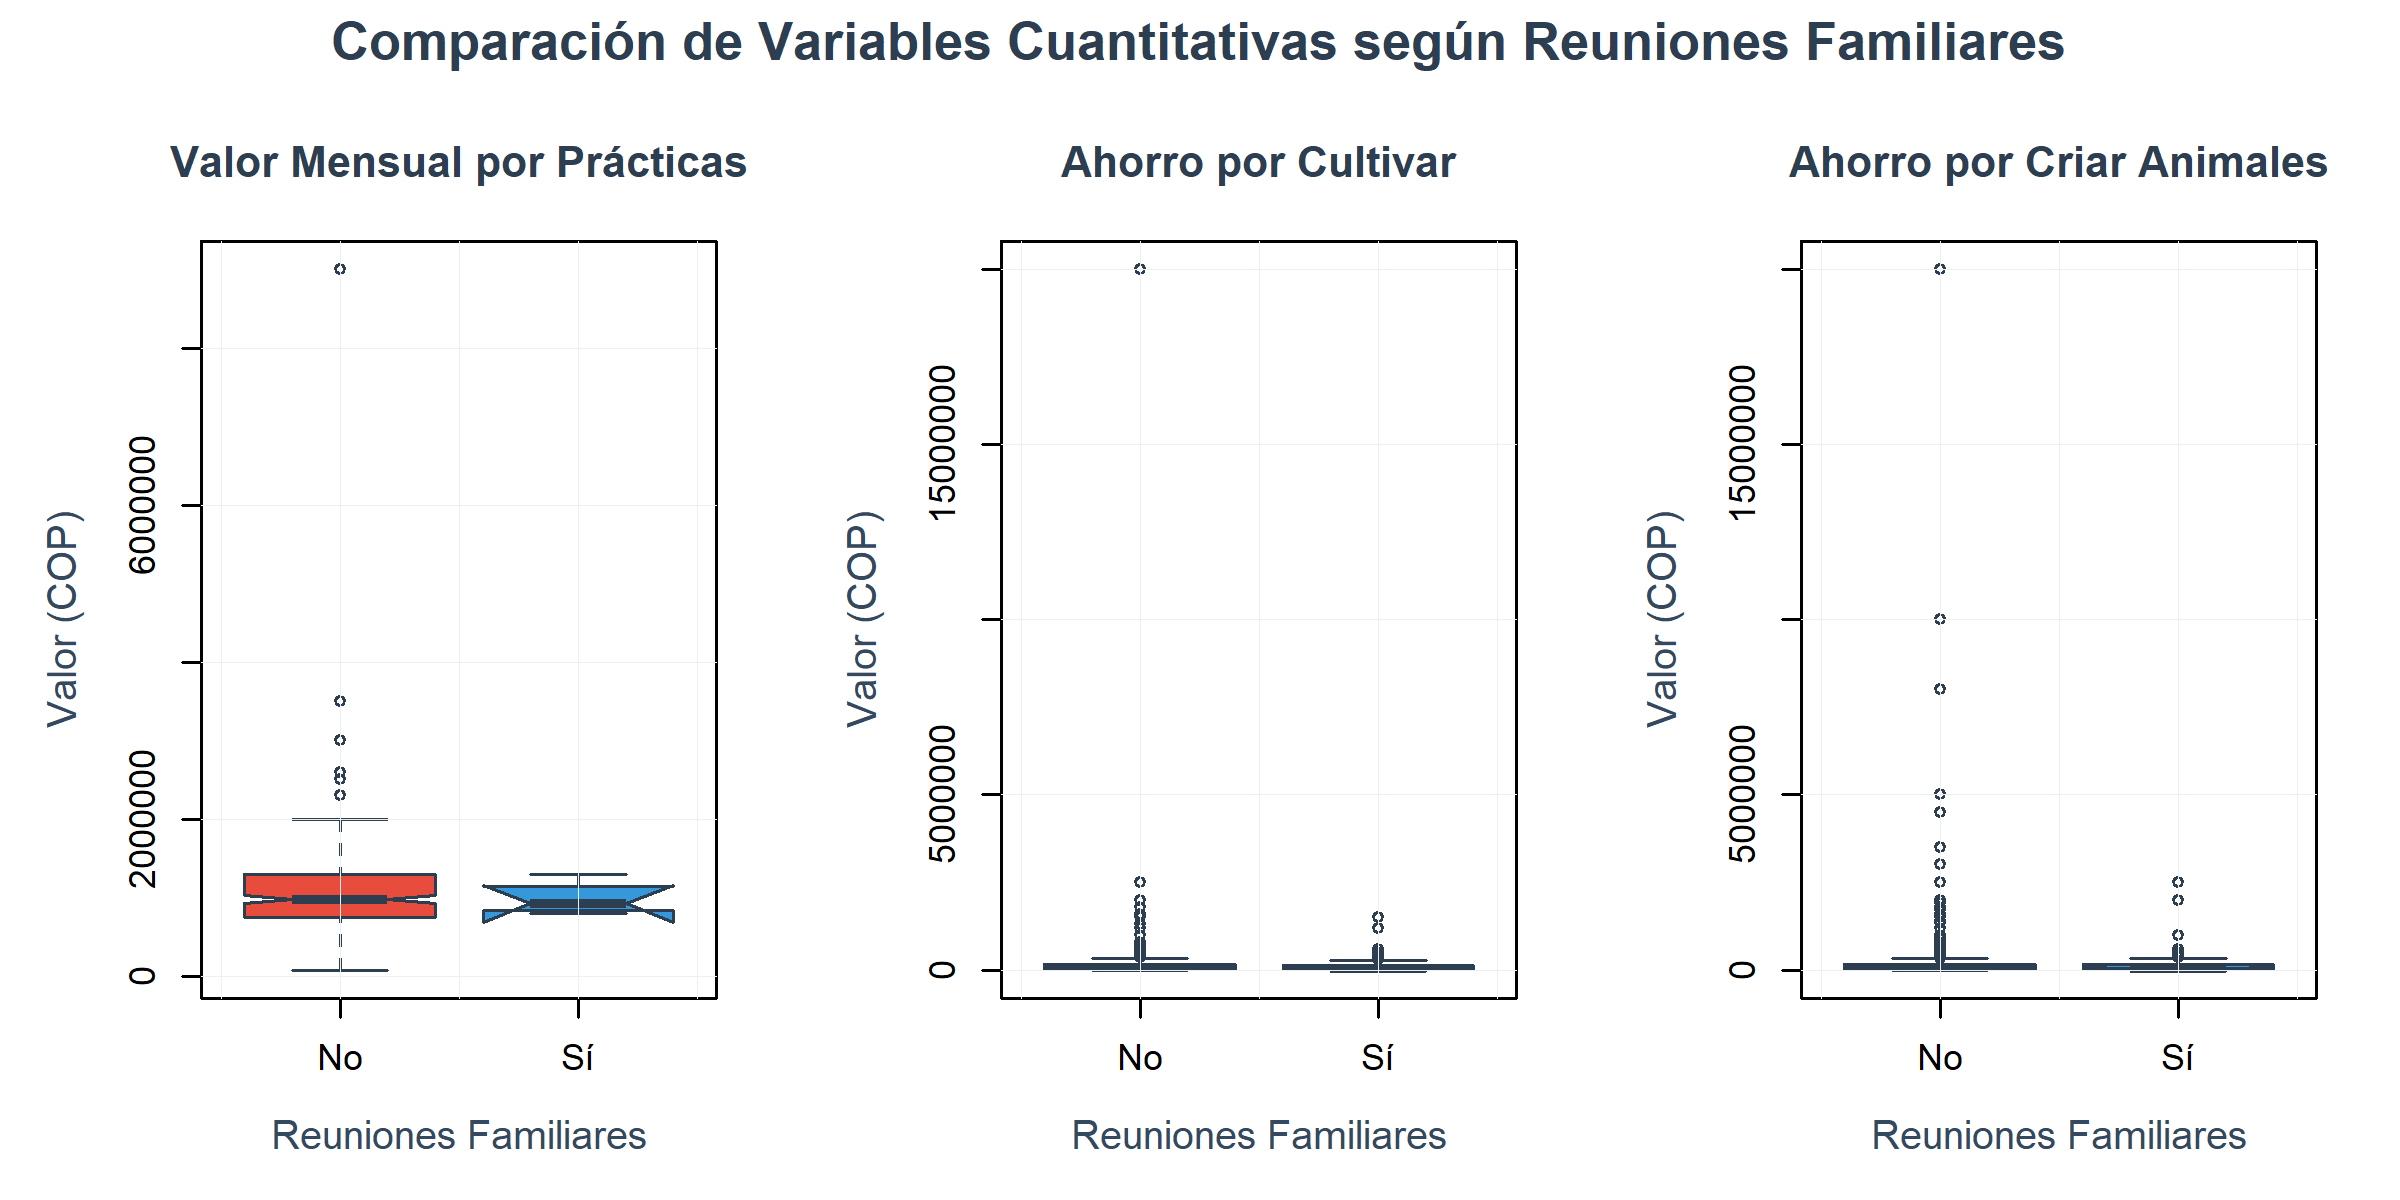
\includegraphics[width=1.0\textwidth]{../Taller 3/plots/comparativo_p3101_boxplots.png}
    \caption{Comparación de Variables Cuantitativas según Reuniones Familiares}
    \label{fig:comparativo_p3101}
\end{figure}

En la Figura \ref{fig:comparativo_p3101} se observan las distribuciones de cada variable cuantitativa separadas por grupo (Sí vs No). Los diagramas de caja permiten visualizar las medianas, cuartiles y valores atípicos de cada grupo, facilitando la comparación visual de las distribuciones. 

Para el \textit{Valor mensual por prácticas} (gráfico izquierdo), se observa que ambos grupos presentan distribuciones similares, sin diferencias visuales marcadas entre quienes asistieron a reuniones familiares y quienes no asistieron. Los diagramas de caja se superponen considerablemente, lo cual es consistente con los resultados de la prueba estadística que no encontró diferencias significativas (p-valor = 0.948).

Para el \textit{Ahorro por cultivar} (gráfico central), aunque existe una ligera diferencia numérica en las medianas entre los grupos, los diagramas de caja muestran una superposición considerable, especialmente en los cuartiles. Esto es consistente con los resultados de la prueba de Mann-Whitney que no encontró diferencias estadísticamente significativas (p-valor = 0.103).

Para el \textit{Ahorro por criar animales} (gráfico derecho), se observa que el grupo que no asistió a reuniones familiares presenta una distribución con valores ligeramente más altos, aunque los diagramas de caja aún muestran cierta superposición. Esta observación visual es consistente con los resultados estadísticos que muestran una diferencia numérica pero no estadísticamente significativa al nivel $\alpha = 0.05$ (p-valor = 0.068).

En general, los resultados visuales y estadísticos son consistentes: no se encontró evidencia estadísticamente significativa de asociación entre la asistencia a reuniones familiares y ninguna de las tres variables económicas analizadas al nivel de significancia de 0.05.

\section*{2. Análisis de Regresión Múltiple}

\subsection*{2.1 Análisis Exploratorio Previo}

El modelo de regresión múltiple propuesto tiene como variable respuesta el \textit{Valor mensual por prácticas o pasantías} (Y) y como variables explicativas el \textit{Ahorro por cultivar} (X$_1$) y el \textit{Ahorro por criar animales} (X$_2$). 

A continuación se presenta el análisis exploratorio de las variables del modelo. La Figura \ref{fig:histogramas} muestra las distribuciones de frecuencia de cada variable del modelo.

\begin{figure}[H]
    \centering
    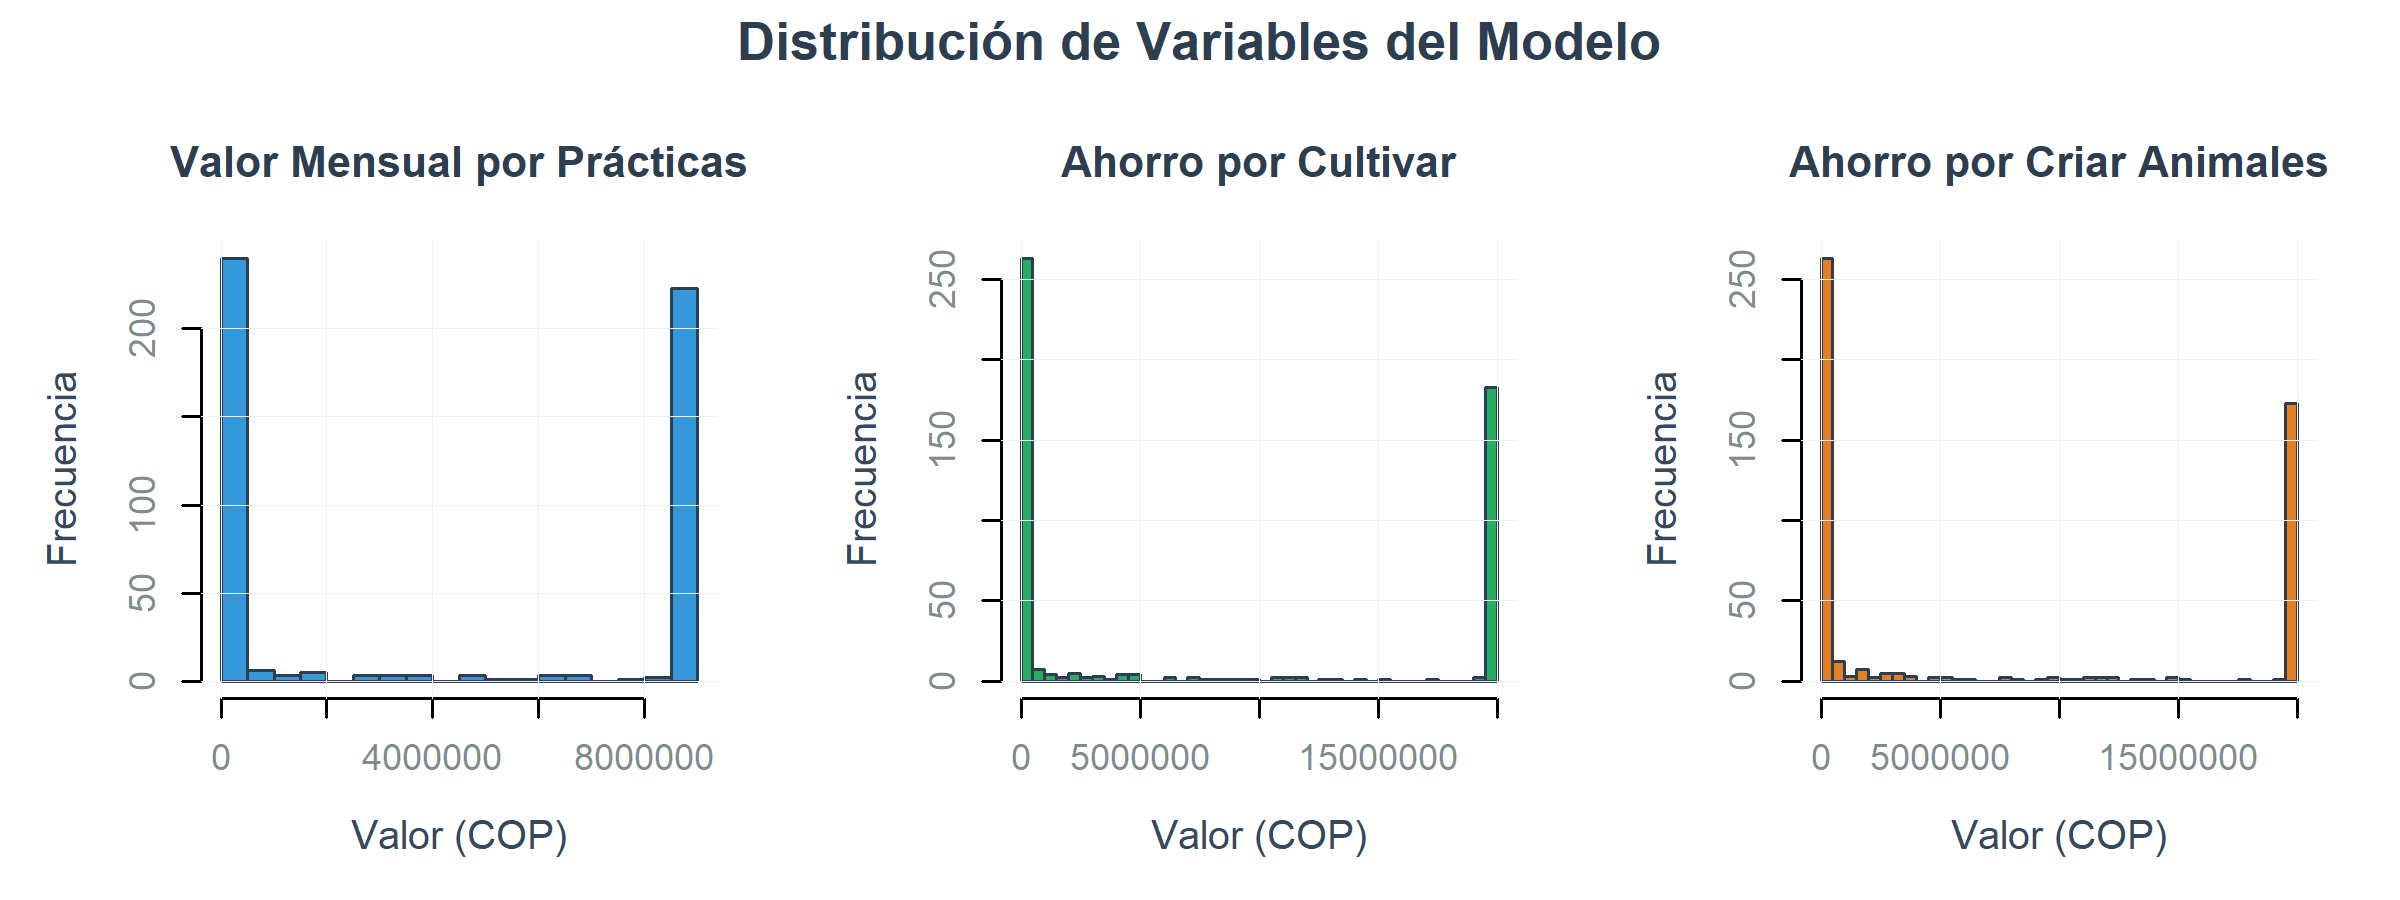
\includegraphics[width=1.0\textwidth]{../Taller 3/plots/exploratorio_histogramas.png}
    \caption{Distribución de Variables del Modelo}
    \label{fig:histogramas}
\end{figure}

En la Figura \ref{fig:histogramas} se observa que las tres variables presentan distribuciones claramente sesgadas hacia la derecha. La variable respuesta (Y: Valor mensual por prácticas) muestra una distribución con una cola larga hacia valores altos, con la mayoría de las observaciones concentradas en valores relativamente bajos (alrededor de 80,000 a 2,000,000 pesos), pero con algunos casos con valores mucho más altos (hasta 9,000,000 pesos). Las variables explicativas (X$_1$: Ahorro por cultivar y X$_2$: Ahorro por criar animales) muestran patrones similares, con distribuciones sesgadas que indican la presencia de algunos valores extremadamente altos. Este tipo de distribución es característico de variables económicas y puede requerir transformaciones logarítmicas para mejorar el cumplimiento de los supuestos del modelo de regresión.

La Figura \ref{fig:dispersion} presenta los diagramas de dispersión entre las variables explicativas y la variable respuesta, incluyendo las rectas de regresión simple para cada relación.

\begin{figure}[H]
    \centering
    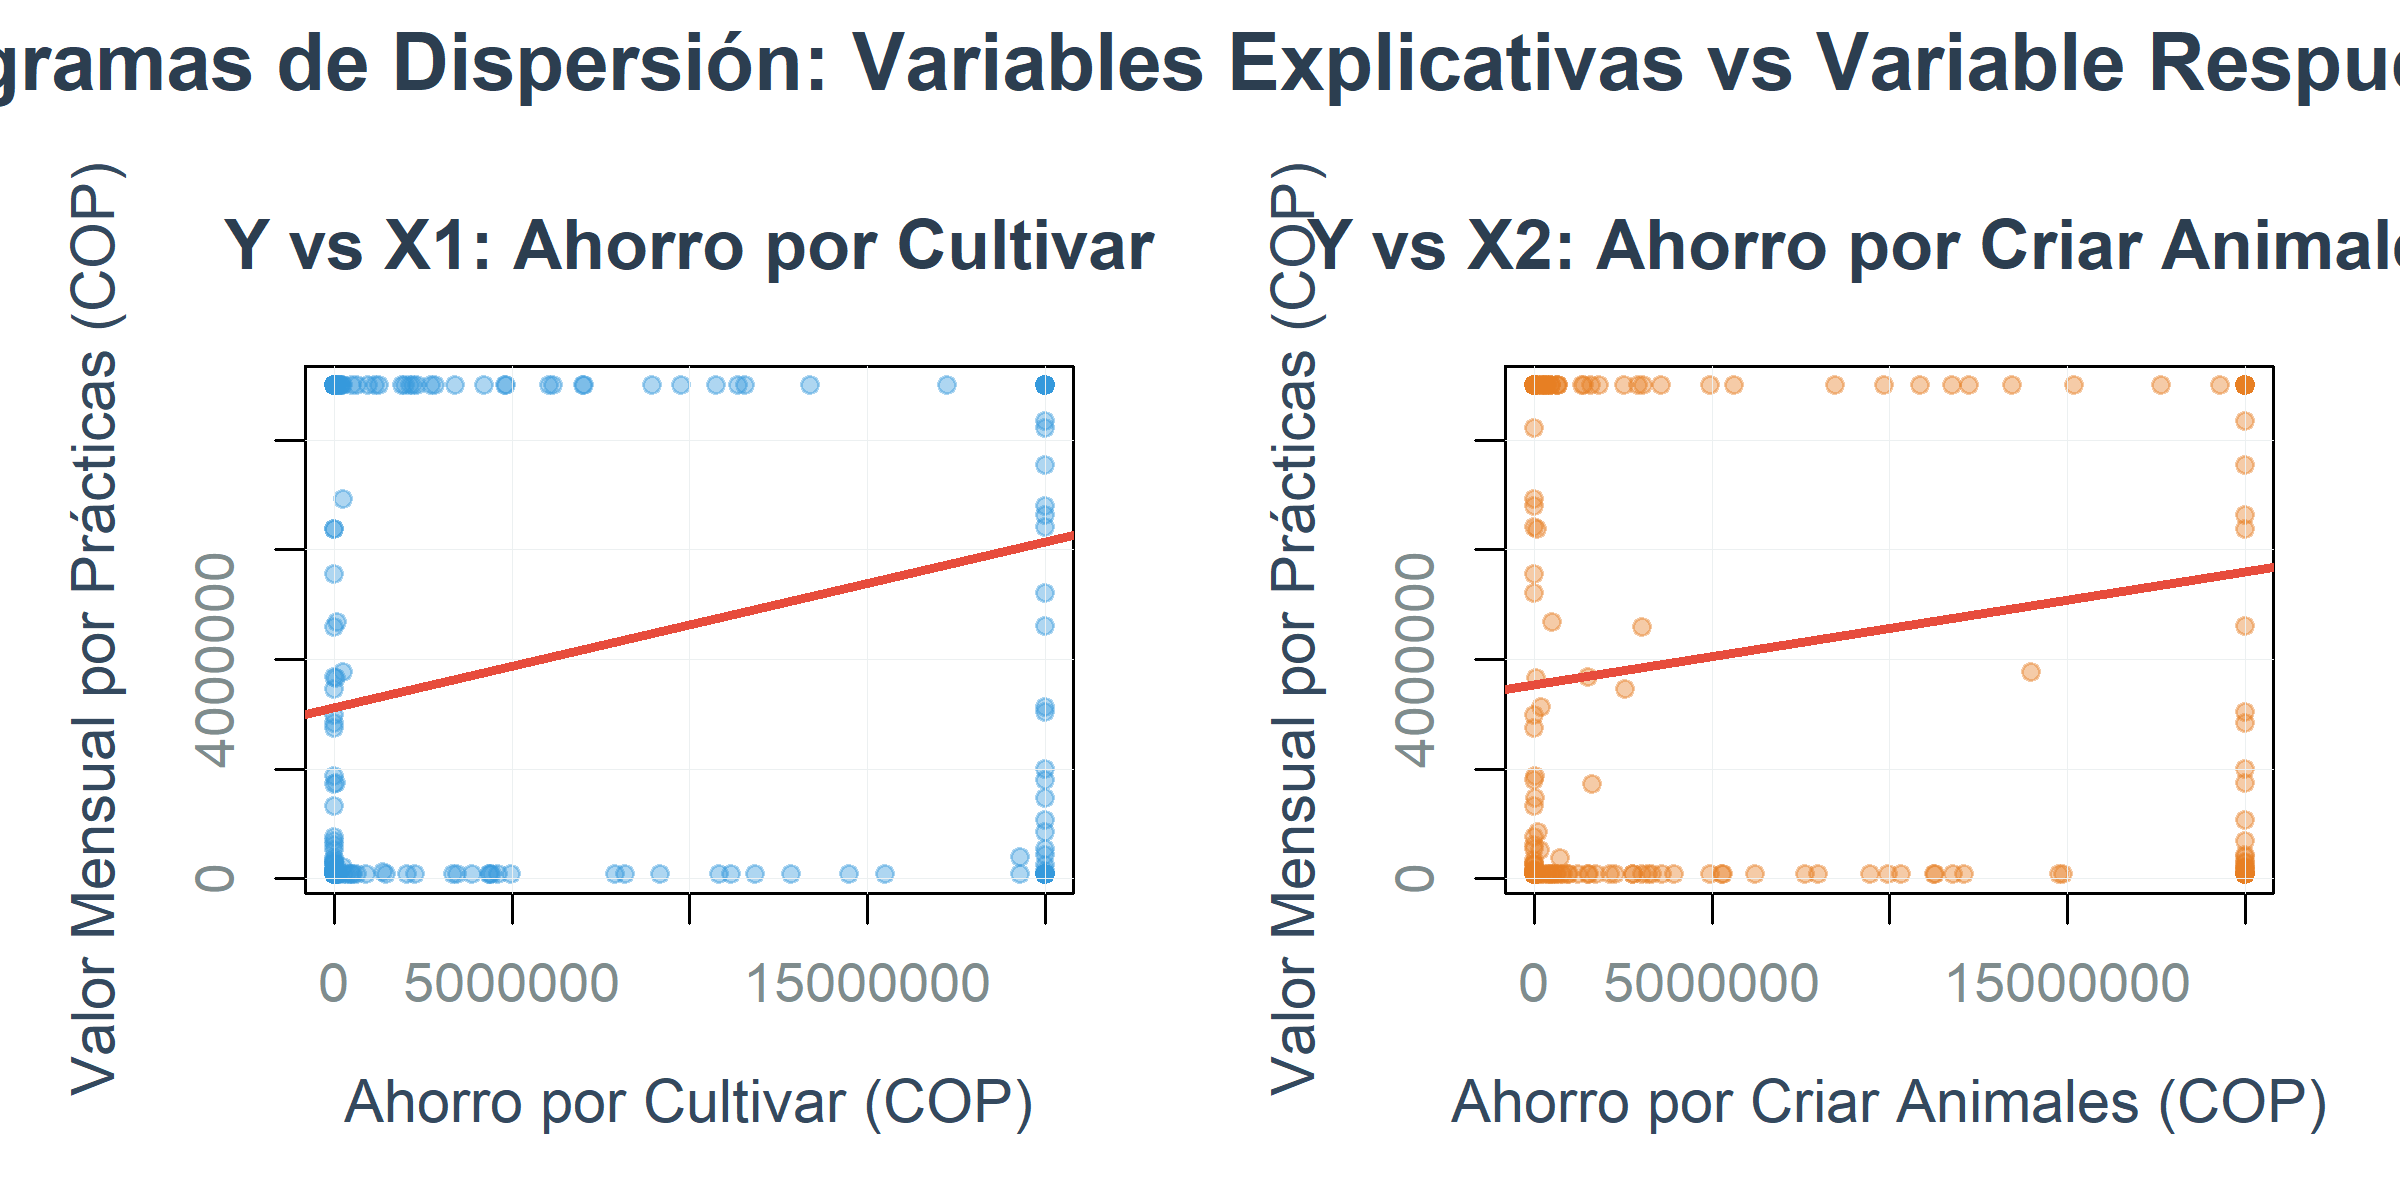
\includegraphics[width=1.0\textwidth]{../Taller 3/plots/exploratorio_dispersion.png}
    \caption{Diagramas de Dispersión: Variables Explicativas vs Variable Respuesta}
    \label{fig:dispersion}
\end{figure}

En la Figura \ref{fig:dispersion} se observan tendencias positivas claras en ambos diagramas de dispersión, lo cual indica relaciones lineales positivas entre las variables explicativas y la variable respuesta. El diagrama Y vs X$_1$ muestra una dispersión relativamente amplia alrededor de la recta de regresión, pero con una pendiente positiva clara, sugiriendo que el ahorro por cultivar tiene una asociación positiva con el valor mensual por prácticas. De manera similar, el diagrama Y vs X$_2$ también muestra una relación positiva, aunque con una pendiente ligeramente menor, lo cual es consistente con los coeficientes de correlación encontrados anteriormente. Ambas relaciones parecen seguir un patrón aproximadamente lineal, lo cual es favorable para el modelo de regresión múltiple propuesto.

\subsection*{2.2 Expectativas del Modelo}

Con base en el análisis exploratorio, se espera encontrar:
\begin{itemize}
    \item Una relación positiva entre el valor mensual por prácticas (Y) y el ahorro por cultivar (X$_1$), dado que ambas representan ingresos o recursos económicos.
    \item Una relación positiva entre el valor mensual por prácticas (Y) y el ahorro por criar animales (X$_2$), por la misma razón.
    \item Que ambas variables explicativas aporten información relevante para explicar la variabilidad en el valor mensual por prácticas.
    \item Posible multicolinealidad entre X$_1$ y X$_2$ si ambas miden conceptos económicos similares, aunque representan fuentes diferentes.
\end{itemize}

\subsection*{2.3 Modelo de Regresión}

\subsubsection*{2.3.1 Planteamiento Formal del Modelo}

El modelo de regresión múltiple se plantea formalmente como:

$$Y = \beta_0 + \beta_1 X_1 + \beta_2 X_2 + \varepsilon$$

Donde:
\begin{itemize}
    \item $Y$ = Valor mensual por prácticas o pasantías (variable respuesta)
    \item $X_1$ = Ahorro por cultivar (variable explicativa 1)
    \item $X_2$ = Ahorro por criar animales (variable explicativa 2)
    \item $\beta_0$ = Intercepto
    \item $\beta_1$ = Coeficiente de regresión para $X_1$
    \item $\beta_2$ = Coeficiente de regresión para $X_2$
    \item $\varepsilon$ = Término de error
\end{itemize}

\subsubsection*{2.3.2 Matriz de Coeficientes del Modelo}

\begin{table}[H]
\centering
\caption{Matriz de Coeficientes del Modelo de Regresión Múltiple}
\label{tab:coeficientes}
\begin{tabular}{|l|c|c|c|c|}
\hline
\textbf{Coeficiente} & \textbf{Estimación} & \textbf{Error Estándar} & \textbf{Estadístico t} & \textbf{Valor-p} \\ \hline
$\beta_0$ (Intercepto) & 2,563,461.55 & 268,708.60 & 9.540 & $6.40 \times 10^{-20}$ *** \\ \hline
$\beta_1$ (X$_1$) & 0.1399 & 0.0192 & 7.271 & $1.39 \times 10^{-12}$ *** \\ \hline
$\beta_2$ (X$_2$) & 0.0844 & 0.0195 & 4.330 & $1.81 \times 10^{-5}$ *** \\ \hline
\end{tabular}
\caption*{Signif. codes: 0 `***' 0.001 `**' 0.01 `*' 0.05 `.' 0.1 ` ' 1}
\end{table}

\subsubsection*{2.3.3 Pruebas de Significancia de Coeficientes Individuales}

Para cada coeficiente se plantean las siguientes hipótesis:

\begin{itemize}
    \item Hipótesis: \quad $H_0: \beta_i = 0$ (el coeficiente no es significativo) \hspace{1cm} $H_1: \beta_i \neq 0$ (el coeficiente es significativo)
    \item Nivel de significancia: $\alpha = 0.05$
    \item Estadístico de Prueba: Prueba t para coeficientes de regresión
\end{itemize}

\textbf{Resultados:}

\begin{itemize}
    \item \textbf{$\beta_0$ (Intercepto):} 
    \begin{itemize}
        \item Estimación: 2,563,461.55
        \item Error estándar: 268,708.60
        \item Estadístico t: 9.540
        \item Valor-p: $6.40 \times 10^{-20}$
        \item Decisión: Rechazar $H_0$. El intercepto es significativo.
        \item Interpretación: El valor esperado del valor mensual por prácticas cuando ambas variables explicativas son cero es de 2,563,461.55 pesos, lo cual es estadísticamente significativo.
    \end{itemize}
    \item \textbf{$\beta_1$ (Coeficiente para X$_1$):} 
    \begin{itemize}
        \item Estimación: 0.1399
        \item Error estándar: 0.0192
        \item Estadístico t: 7.271
        \item Valor-p: $1.39 \times 10^{-12}$
        \item Decisión: Rechazar $H_0$. El coeficiente para el ahorro por cultivar es significativo.
        \item Interpretación: Manteniendo constante el ahorro por criar animales, un aumento de 1 peso en el ahorro por cultivar se asocia con un aumento promedio de 0.1399 pesos en el valor mensual por prácticas. Esto indica que el ahorro por cultivar tiene un efecto positivo y significativo sobre el valor mensual por prácticas.
    \end{itemize}
    \item \textbf{$\beta_2$ (Coeficiente para X$_2$):} 
    \begin{itemize}
        \item Estimación: 0.0844
        \item Error estándar: 0.0195
        \item Estadístico t: 4.330
        \item Valor-p: $1.81 \times 10^{-5}$
        \item Decisión: Rechazar $H_0$. El coeficiente para el ahorro por criar animales es significativo.
        \item Interpretación: Manteniendo constante el ahorro por cultivar, un aumento de 1 peso en el ahorro por criar animales se asocia con un aumento promedio de 0.0844 pesos en el valor mensual por prácticas. Esto indica que el ahorro por criar animales tiene un efecto positivo y significativo sobre el valor mensual por prácticas, aunque el efecto es menor que el del ahorro por cultivar.
    \end{itemize}
\end{itemize}

\subsubsection*{2.3.4 Prueba de Significancia Global del Modelo}

\begin{itemize}
    \item Hipótesis: \quad $H_0: \beta_1 = \beta_2 = 0$ (ninguna variable explicativa es útil) \hspace{1cm} $H_1:$ Al menos un $\beta_i \neq 0$ (al menos una variable explicativa es útil)
    \item Nivel de significancia: $\alpha = 0.05$
    \item Estadístico de Prueba: Prueba F global
\end{itemize}

\begin{tabular}{|m{7cm}|m{7cm}|}
\hline
\textbf{Estadístico Empleado} & Prueba F global \\ \hline
\textbf{Fórmula del estadístico} & $F = \frac{MSR}{MSE} = \frac{R^2/k}{(1-R^2)/(n-k-1)}$ \\ \hline
\textbf{Nombre Parámetro} & \textbf{Valor} \\ \hline
Estadístico F & 40.77 \\ \hline
Grados de libertad (numerador) & 2 \\ \hline
Grados de libertad (denominador) & 497 \\ \hline
Valor-p & $< 2.2 \times 10^{-16}$ \\ \hline
R$^2$ (coeficiente de determinación) & 0.141 \\ \hline
R$^2$ ajustado & 0.1375 \\ \hline
Error estándar residual & 4,031,070 \\ \hline
\end{tabular}

\begin{itemize}
    \item Regla de decisión: Rechazar $H_0$ si p-valor $< 0.05$
    \item Decisión: Rechazar $H_0$
    \item Conclusión: Con un nivel de significancia de 0.05, la evidencia sugiere que el modelo es significativo globalmente. Al menos una variable explicativa aporta información relevante para explicar la variabilidad en el valor mensual por prácticas. El modelo explica el 14.1\% de la variabilidad total (R$^2$ = 0.141).
\end{itemize}

\subsubsection*{2.3.5 Análisis de Varianza (ANOVA)}

\begin{itemize}
    \item Hipótesis: \quad $H_0:$ Todos los coeficientes de regresión son cero (modelo no útil) \hspace{1cm} $H_1:$ Al menos un coeficiente de regresión es diferente de cero
    \item Nivel de significancia: $\alpha = 0.05$
    \item Estadístico de Prueba: $\chi^2$ / Prueba F
\end{itemize}

\begin{table}[H]
\centering
\caption{Tabla ANOVA del Modelo de Regresión}
\label{tab:anova}
\begin{tabular}{|l|c|c|c|c|c|}
\hline
\textbf{Fuente} & \textbf{gl} & \textbf{Suma de Cuadrados} & \textbf{Cuadrados Medios} & \textbf{F} & \textbf{Valor-p} \\ \hline
X$_1$ & 1 & 1,020,488,415,971,762 & 1,020,488,415,971,762 & 62.80 & $1.51 \times 10^{-15}$ *** \\ \hline
X$_2$ & 1 & 304,601,872,025,046 & 304,601,872,025,046 & 18.75 & $1.81 \times 10^{-5}$ *** \\ \hline
Residuales & 497 & 8,076,013,748,592,473 & 16,249,524,645,055.3 & - & - \\ \hline
\end{tabular}
\caption*{Signif. codes: 0 `***' 0.001 `**' 0.01 `*' 0.05 `.' 0.1 ` ' 1}
\end{table}

\begin{itemize}
    \item Regla de decisión: Rechazar $H_0$ si p-valor $< 0.05$
    \item Decisión: Rechazar $H_0$ para ambas variables explicativas
    \item Interpretación: La tabla ANOVA descompone la variabilidad total en variabilidad explicada por cada variable explicativa y variabilidad no explicada (residual). Tanto X$_1$ como X$_2$ son significativos individualmente (X$_1$: F = 62.80, p-valor $= 1.51 \times 10^{-15}$; X$_2$: F = 18.75, p-valor $= 1.81 \times 10^{-5}$), lo que confirma que ambas variables explicativas aportan información relevante al modelo. El ahorro por cultivar (X$_1$) aporta más variabilidad explicada (Suma de Cuadrados = 1,020,488,415,971,762) que el ahorro por criar animales (X$_2$: Suma de Cuadrados = 304,601,872,025,046), lo cual es consistente con el mayor coeficiente de correlación encontrado entre Y y X$_1$ en el análisis de correlación.
\end{itemize}

\subsection*{2.4 Validación de Supuestos}

Se evaluaron gráficamente y analíticamente los supuestos del modelo de regresión múltiple: linealidad, independencia, homocedasticidad y normalidad de los errores.

\subsubsection*{2.4.1 Supuesto de Linealidad}

\begin{itemize}
    \item Hipótesis: \quad $H_0:$ La relación entre variables es lineal \hspace{2cm} $H_1:$ La relación entre variables no es lineal
    \item Nivel de significancia: $\alpha = 0.05$
    \item Método de Evaluación: Inspección gráfica de residuos vs valores ajustados
\end{itemize}

Para evaluar el supuesto de linealidad, se analizan los gráficos de residuos vs valores ajustados. La Figura \ref{fig:linealidad} presenta los gráficos de residuos estandarizados y residuos vs valores ajustados.

\begin{figure}[H]
    \centering
    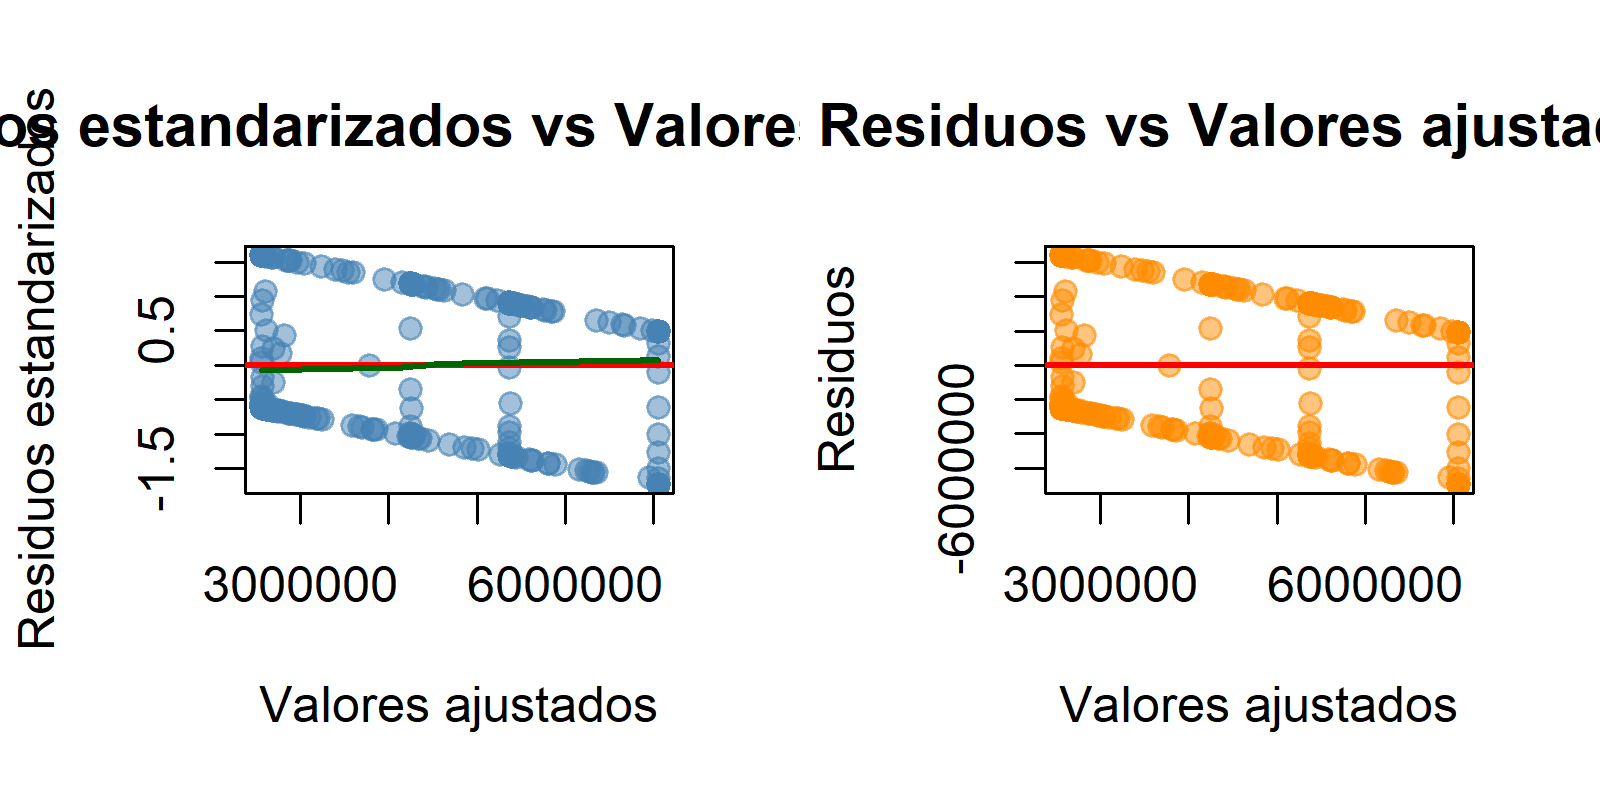
\includegraphics[width=1.0\textwidth]{../Taller 3/plots/validacion_linealidad.png}
    \caption{Validación de Linealidad: Gráficos de Residuos}
    \label{fig:linealidad}
\end{figure}

En la Figura \ref{fig:linealidad} se observa que los residuos estandarizados (gráfico izquierdo) se distribuyen de manera relativamente aleatoria alrededor de la línea horizontal en cero, sin mostrar patrones sistemáticos claros como curvas o tendencias. La línea de suavizado (en verde) muestra una ligera variación pero sin patrones marcados de no linealidad. El gráfico de residuos vs valores ajustados (gráfico derecho) también muestra un patrón relativamente aleatorio, aunque con una mayor dispersión en los valores más altos de los valores ajustados. Esta mayor variabilidad en los valores altos podría indicar una ligera heterocedasticidad o podría ser simplemente un efecto del menor número de observaciones en esos rangos. En general, el supuesto de linealidad se cumple aproximadamente, aunque se recomienda considerar transformaciones si se detectan otros problemas en los supuestos.

\subsubsection*{2.4.2 Supuesto de Independencia}

\begin{itemize}
    \item Hipótesis: \quad $H_0:$ Los residuos son independientes (no hay autocorrelación) \hspace{1cm} $H_1:$ Los residuos no son independientes (hay autocorrelación)
    \item Nivel de significancia: $\alpha = 0.05$
    \item Estadístico de Prueba: Prueba de Durbin-Watson
\end{itemize}

\begin{tabular}{|m{7cm}|m{7cm}|}
\hline
\textbf{Estadístico Empleado} & Prueba de Durbin-Watson \\ \hline
\textbf{Nombre Parámetro} & \textbf{Valor} \\ \hline
Estadístico DW & 1.9726 \\ \hline
Valor-p & 0.752 \\ \hline
\end{tabular}

\begin{itemize}
    \item Regla de decisión: Rechazar $H_0$ si p-valor $< 0.05$
    \item Decisión: No rechazar $H_0$
    \item Conclusión: No hay evidencia de autocorrelación en los residuos. El supuesto de independencia se cumple.
\end{itemize}

Para evaluar el supuesto de independencia de los residuos, se analiza la secuencia de residuos a lo largo del orden de observación. La Figura \ref{fig:independencia} muestra los residuos estandarizados vs el orden de observación.

\begin{figure}[H]
    \centering
    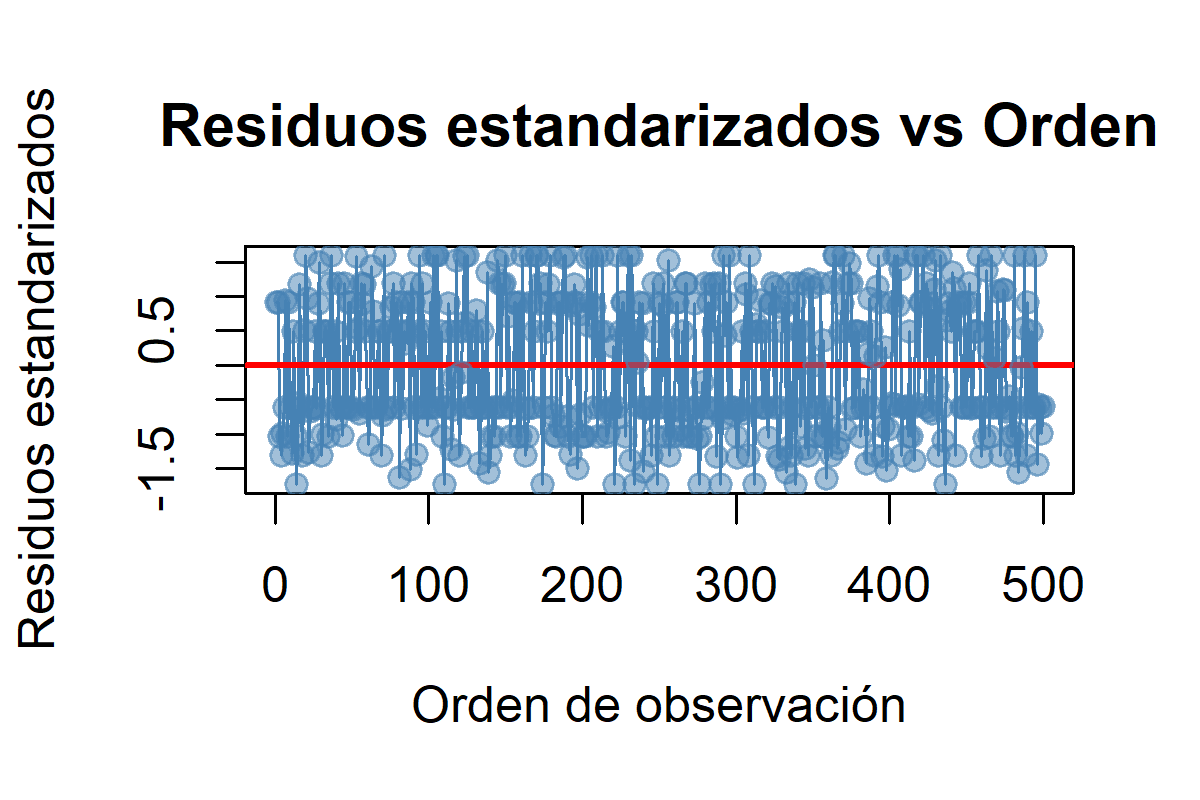
\includegraphics[width=0.8\textwidth]{../Taller 3/plots/validacion_independencia.png}
    \caption{Validación de Independencia: Residuos vs Orden}
    \label{fig:independencia}
\end{figure}

En la Figura \ref{fig:independencia} se observa que los residuos estandarizados fluctúan de manera aleatoria alrededor de la línea horizontal en cero a lo largo del orden de observación, sin mostrar patrones sistemáticos como tendencias crecientes o decrecientes, ciclos o agrupamientos. Esta distribución aleatoria indica que no hay evidencia de autocorrelación en los residuos, lo cual es consistente con los resultados de la prueba de Durbin-Watson (DW = 1.9726, p-valor = 0.752). El supuesto de independencia se cumple, lo cual es esperado dado que las observaciones provienen de diferentes hogares y no deberían estar correlacionadas temporal o espacialmente de manera sistemática.

\subsubsection*{2.4.3 Supuesto de Homocedasticidad}

\begin{itemize}
    \item Hipótesis: \quad $H_0:$ Varianza constante de los errores (homocedasticidad) \hspace{1cm} $H_1:$ Varianza no constante de los errores (heterocedasticidad)
    \item Nivel de significancia: $\alpha = 0.05$
    \item Estadístico de Prueba: Prueba de Breusch-Pagan
\end{itemize}

\begin{tabular}{|m{7cm}|m{7cm}|}
\hline
\textbf{Estadístico Empleado} & Prueba de Breusch-Pagan \\ \hline
\textbf{Nombre Parámetro} & \textbf{Valor} \\ \hline
Estadístico LM & 0.0679 \\ \hline
Valor-p & 0.967 \\ \hline
\end{tabular}

\begin{itemize}
    \item Regla de decisión: Rechazar $H_0$ si p-valor $< 0.05$
    \item Decisión: No rechazar $H_0$
    \item Conclusión: No hay evidencia de heterocedasticidad. El supuesto de homocedasticidad se cumple.
\end{itemize}

Para evaluar el supuesto de homocedasticidad (varianza constante de los errores), se utiliza el gráfico de escala-localización, el cual muestra la raíz cuadrada del valor absoluto de los residuos estandarizados vs los valores ajustados. La Figura \ref{fig:homocedasticidad} presenta este gráfico.

\begin{figure}[H]
    \centering
    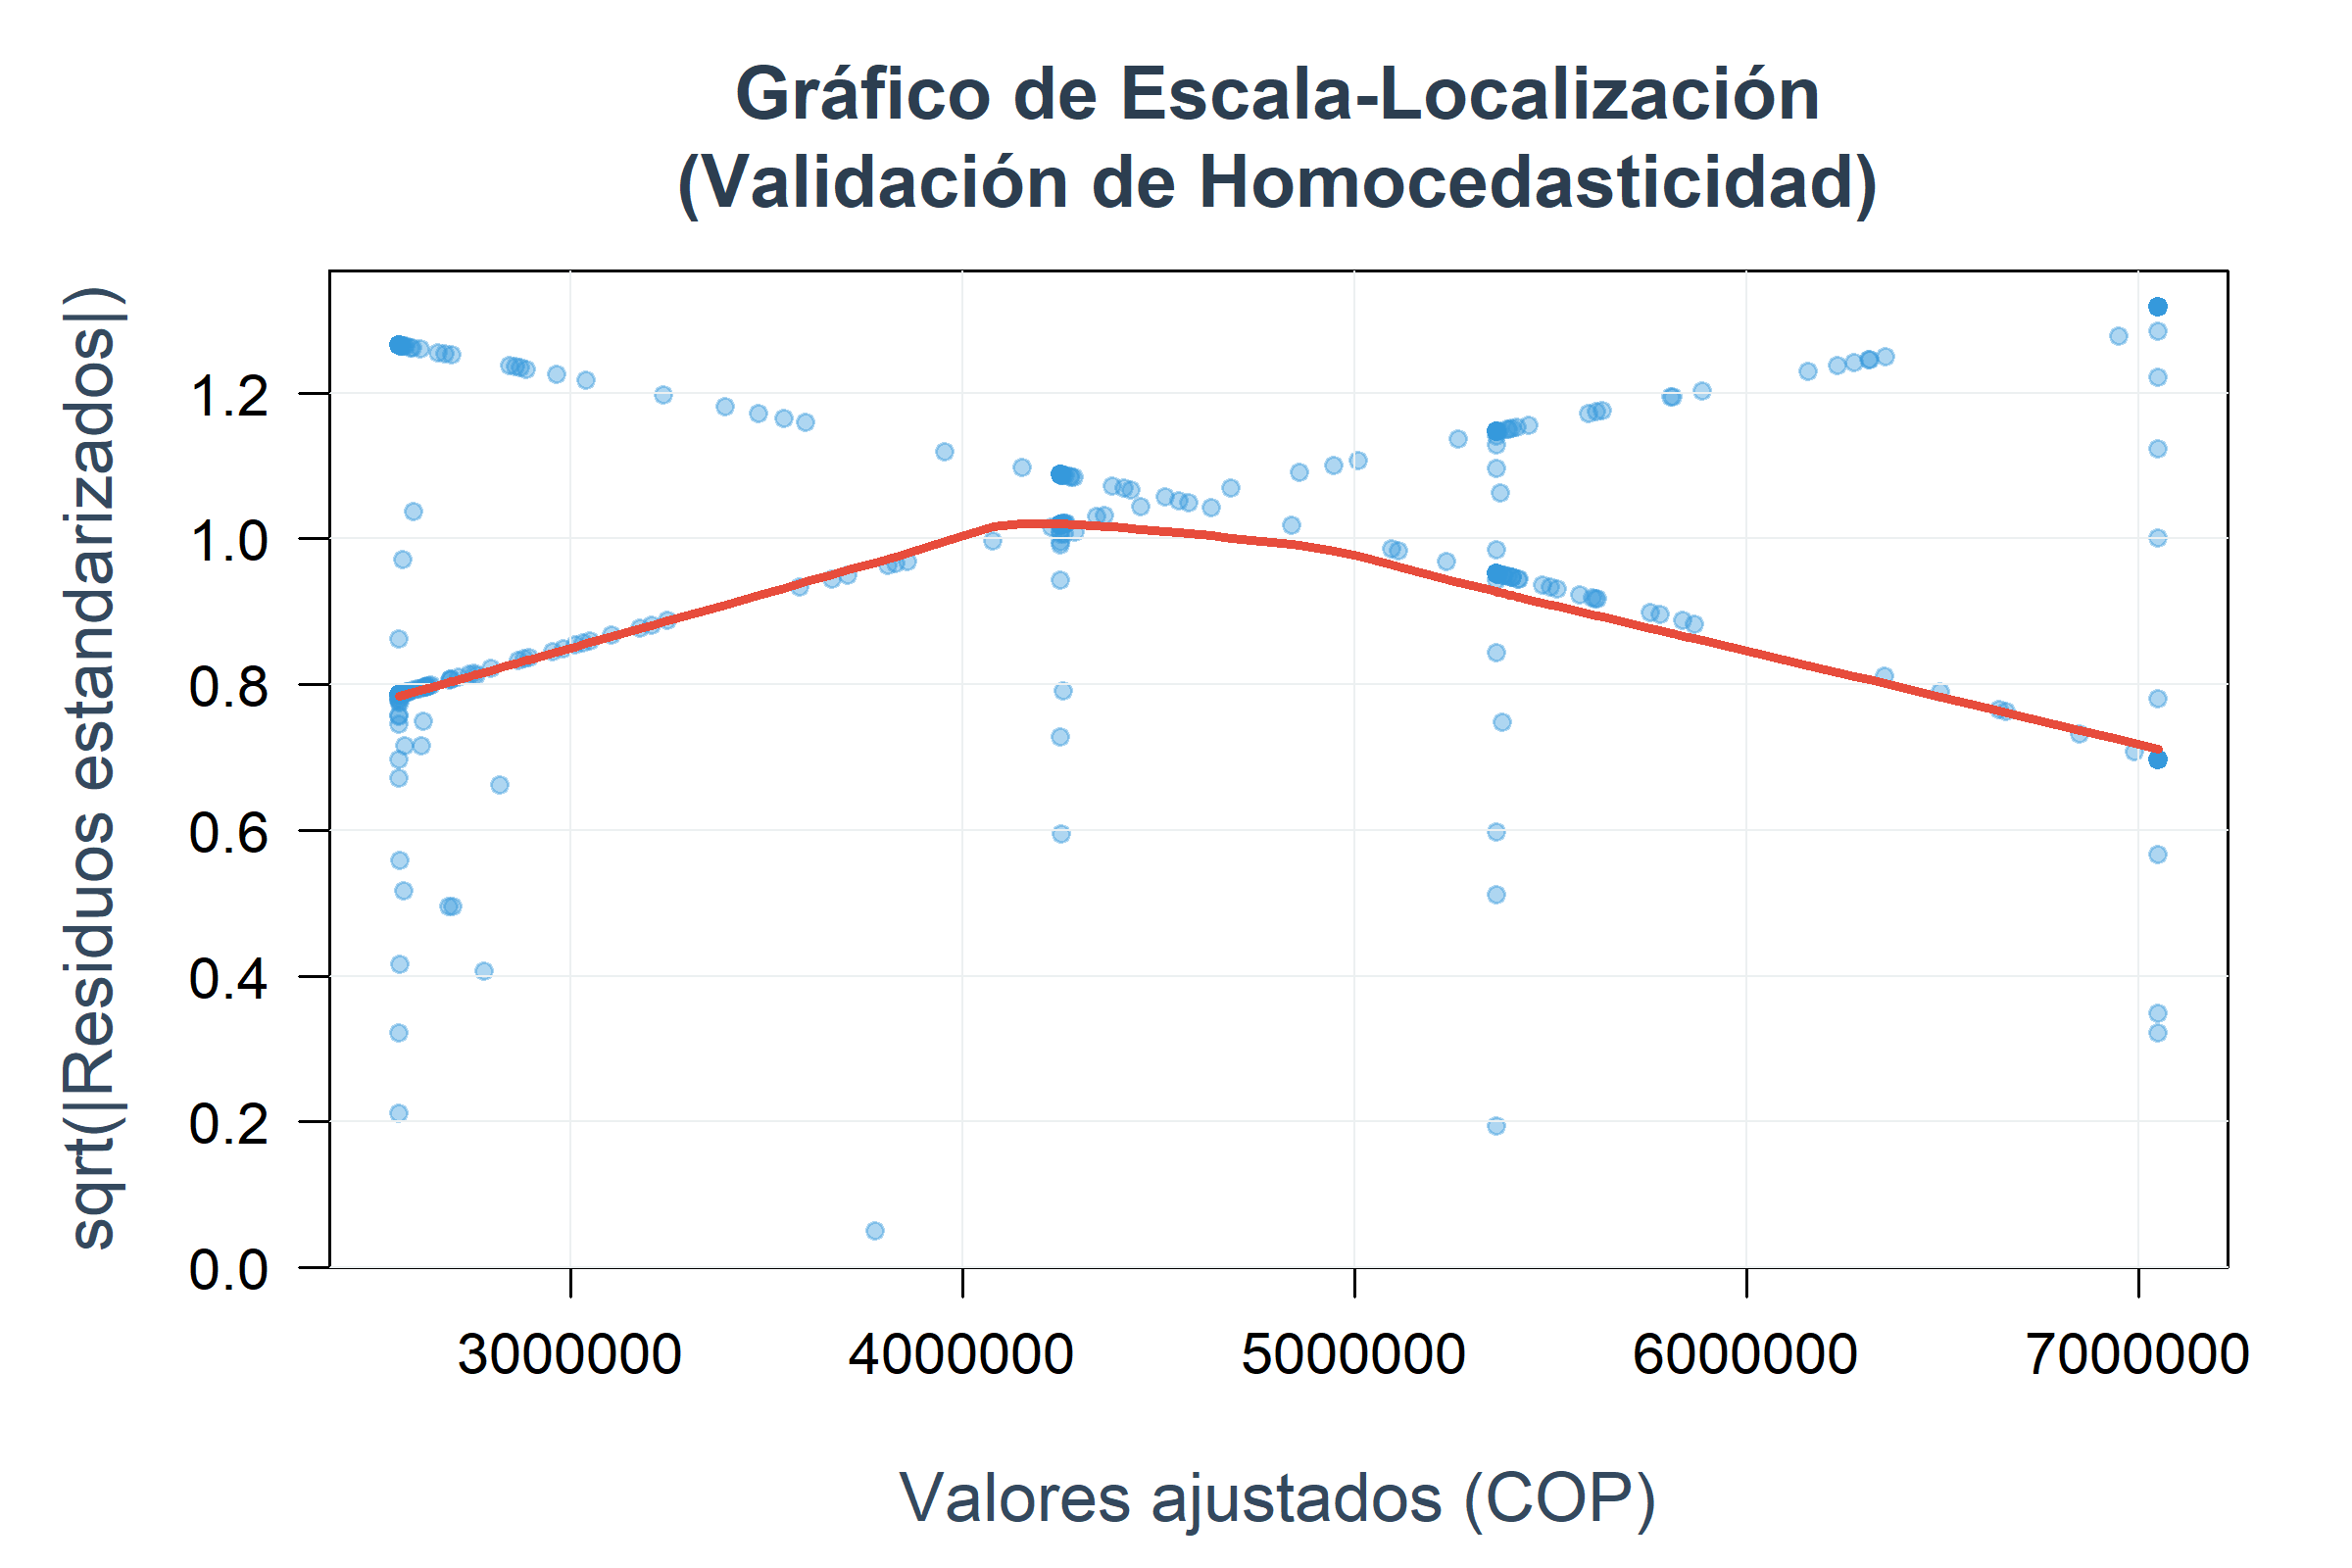
\includegraphics[width=0.8\textwidth]{../Taller 3/plots/validacion_homocedasticidad.png}
    \caption{Validación de Homocedasticidad: Gráfico de Escala-Localización}
    \label{fig:homocedasticidad}
\end{figure}

En la Figura \ref{fig:homocedasticidad} se observa que la línea de suavizado (en rojo) se mantiene relativamente horizontal a lo largo del rango de valores ajustados, con algunas variaciones menores pero sin una tendencia clara de aumento o disminución sistemática. Si existiera heterocedasticidad, se esperaría ver una tendencia marcada en esta línea, ya sea creciente (indicando que la varianza aumenta con los valores ajustados) o decreciente (indicando que la varianza disminuye). La ausencia de una tendencia clara, junto con el resultado de la prueba de Breusch-Pagan (LM = 0.0679, p-valor = 0.967), confirma que el supuesto de homocedasticidad se cumple. Esto indica que la varianza de los errores es constante a lo largo de todos los valores de las variables explicativas, lo cual es necesario para que los intervalos de confianza y las pruebas de hipótesis sean válidos.

\subsubsection*{2.4.4 Supuesto de Normalidad de los Errores}

\begin{itemize}
    \item Hipótesis: \quad $H_0:$ Los errores siguen una distribución normal \hspace{2cm} $H_1:$ Los errores no siguen una distribución normal
    \item Nivel de significancia: $\alpha = 0.05$
    \item Estadístico de Prueba: Prueba de Shapiro-Wilk
\end{itemize}

\begin{tabular}{|m{7cm}|m{7cm}|}
\hline
\textbf{Estadístico Empleado} & Prueba de Shapiro-Wilk \\ \hline
\textbf{Nombre Parámetro} & \textbf{Valor} \\ \hline
Estadístico W & 0.9123 \\ \hline
Valor-p & $2.03 \times 10^{-16}$ \\ \hline
\end{tabular}

\begin{itemize}
    \item Regla de decisión: Rechazar $H_0$ si p-valor $< 0.05$
    \item Decisión: Rechazar $H_0$
    \item Conclusión: Los residuos no siguen una distribución normal. El supuesto de normalidad no se cumple.
\end{itemize}

Para evaluar el supuesto de normalidad de los errores, se utilizan tanto el gráfico Q-Q (quantil-quantil) como el histograma de los residuos estandarizados. La Figura \ref{fig:normalidad} muestra ambos gráficos.

\begin{figure}[H]
    \centering
    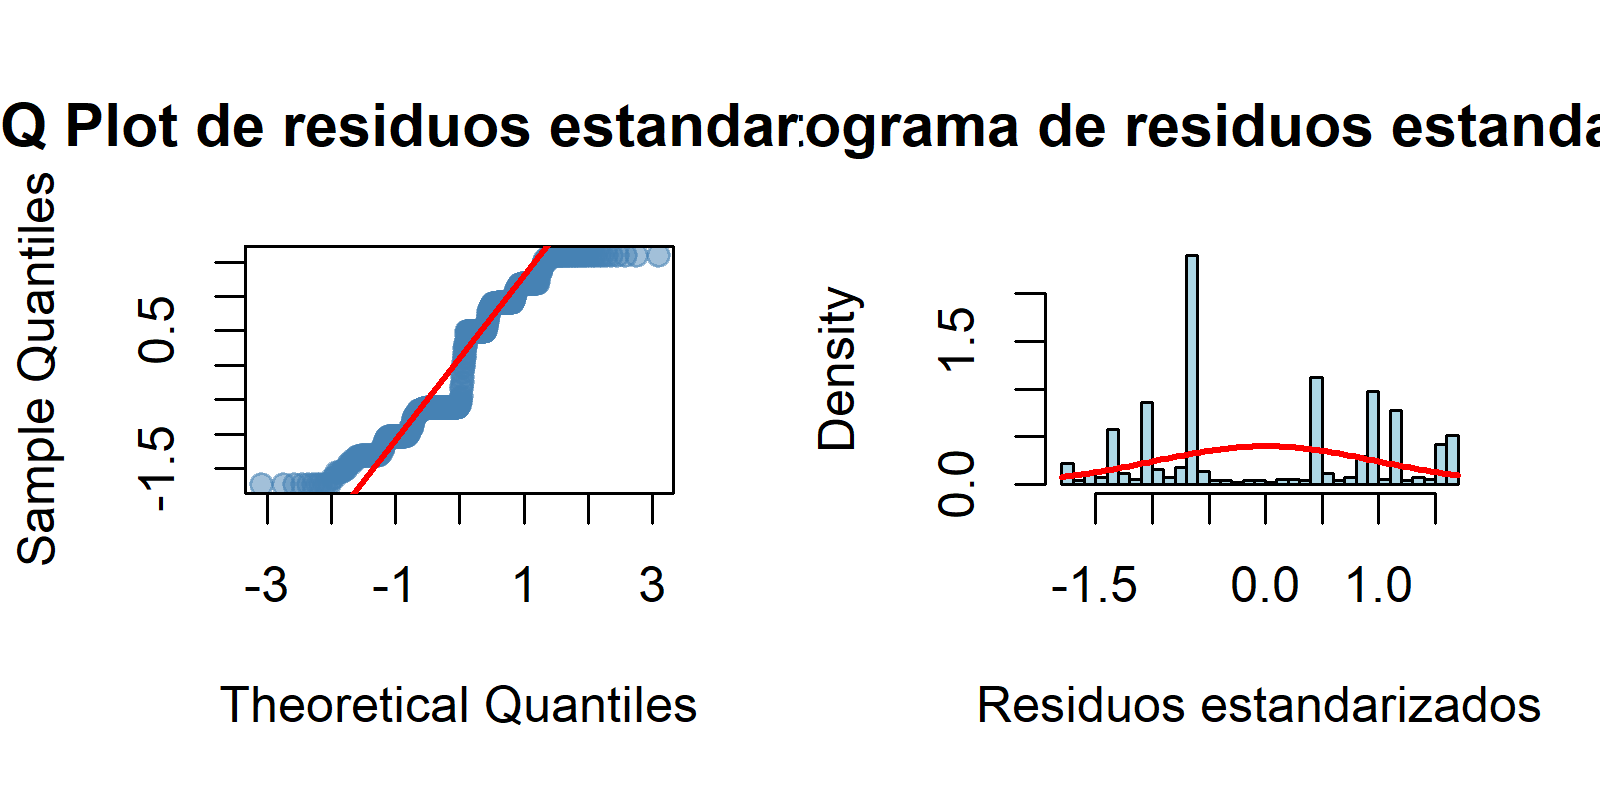
\includegraphics[width=1.0\textwidth]{../Taller 3/plots/validacion_normalidad.png}
    \caption{Validación de Normalidad: Q-Q Plot e Histograma}
    \label{fig:normalidad}
\end{figure}

En la Figura \ref{fig:normalidad} se observa claramente que los residuos no siguen una distribución normal. En el Q-Q plot (gráfico izquierdo), los puntos se desvían notablemente de la línea de referencia (en rojo), especialmente en las colas de la distribución. Los valores en los extremos inferiores (cuantiles teóricos negativos) y superiores (cuantiles teóricos positivos) se alejan significativamente de la línea, indicando que la distribución tiene colas más pesadas que la distribución normal. El histograma (gráfico derecho) confirma este hallazgo, mostrando una distribución que, aunque parece aproximadamente simétrica alrededor de cero, presenta colas más pesadas y posiblemente una forma más puntiaguda (leptocúrtica) o más plana (platicúrtica) que la distribución normal teórica (superpuesta en rojo). Estos hallazgos visuales son consistentes con el resultado de la prueba de Shapiro-Wilk (W = 0.9123, p-valor $< 0.001$), que rechaza la hipótesis nula de normalidad. Sin embargo, dado el tamaño de muestra grande (n = 500) y el cumplimiento de los demás supuestos críticos (independencia y homocedasticidad), el modelo sigue siendo válido debido al Teorema del Límite Central, aunque los intervalos de confianza pueden ser menos precisos que si se cumpliera completamente el supuesto de normalidad.

\subsubsection*{2.4.5 Tabla Resumen de Validación de Supuestos}

\begin{table}[H]
\centering
\footnotesize
\caption{Tabla Resumen de Validación de Supuestos del Modelo}
\label{tab:supuestos}
\begin{tabularx}{\linewidth}{|>{\raggedright\arraybackslash}X|>{\raggedright\arraybackslash}X|>{\centering\arraybackslash}X|>{\centering\arraybackslash}X|>{\raggedright\arraybackslash}X|>{\centering\arraybackslash}X|}
\hline
\textbf{Supuesto} & \textbf{Prueba} & \textbf{Estadístico} & \textbf{Valor-p} & \textbf{Decisión} & \textbf{Cumplimiento} \\ \hline
Linealidad & Inspección gráfica & N/A (gráfico) & N/A & Evaluar gráficamente & Aproximadamente \\ \hline
Independencia & Durbin-Watson & 1.9726 & 0.752 & No rechazar $H_0$ & Sí \\ \hline
Homocedasticidad & Breusch-Pagan & 0.0679 & 0.967 & No rechazar $H_0$ & Sí \\ \hline
Normalidad de errores & Shapiro-Wilk & 0.9123 & $2.03 \times 10^{-16}$ & Rechazar $H_0$ & No \\ \hline
\end{tabularx}
\end{table}
\normalsize

\textbf{Comentarios sobre cumplimiento de supuestos:}

\begin{itemize}
    \item \textbf{Linealidad:} La inspección gráfica de los residuos vs valores ajustados sugiere un patrón relativamente aleatorio alrededor de cero, indicando que el supuesto de linealidad se cumple aproximadamente.
    \item \textbf{Independencia:} La prueba de Durbin-Watson no muestra evidencia de autocorrelación (p-valor = 0.752). El supuesto de independencia se cumple.
    \item \textbf{Homocedasticidad:} La prueba de Breusch-Pagan no muestra evidencia de heterocedasticidad (p-valor = 0.967). El supuesto de homocedasticidad se cumple.
    \item \textbf{Normalidad:} La prueba de Shapiro-Wilk indica que los residuos no siguen una distribución normal (p-valor $< 0.001$). El supuesto de normalidad \textbf{no se cumple}. Esta violación puede afectar los intervalos de confianza y las pruebas de hipótesis, especialmente en muestras pequeñas. Sin embargo, dado el tamaño de muestra (n = 500), los resultados del modelo son robustos a esta violación debido al Teorema del Límite Central.
\end{itemize}

\subsection*{2.5 Transformaciones}

Evaluando la necesidad de transformaciones, se detectó una violación del supuesto de normalidad de los errores. Se consideró aplicar una transformación logarítmica a las variables.

\textbf{Opción evaluada:} Transformación logarítmica
$$log(Y+1) = \beta_0 + \beta_1 log(X_1+1) + \beta_2 log(X_2+1) + \varepsilon$$

\textbf{Justificación técnica:} Las variables económicas suelen tener distribuciones sesgadas que se normalizan con transformación logarítmica. Esta transformación también puede ayudar a estabilizar la varianza de los errores.

\textbf{Resultados del modelo transformado:}
\begin{itemize}
    \item Prueba de Breusch-Pagan (modelo transformado): Valor-p = 0.990
    \item Prueba de Shapiro-Wilk (modelo transformado): Valor-p $< 0.001$
\end{itemize}

\textbf{Decisión técnica:} La transformación logarítmica no mejora significativamente el cumplimiento del supuesto de normalidad. Aunque mejora la homocedasticidad, la normalidad sigue siendo rechazada. 

Dado que:
\begin{itemize}
    \item El tamaño de muestra es grande (n = 500), lo que proporciona robustez a la violación del supuesto de normalidad
    \item Los supuestos de independencia y homocedasticidad se cumplen
    \item La transformación logarítmica no resuelve completamente el problema de normalidad
\end{itemize}

Se recomienda mantener el modelo original sin transformaciones, reconociendo la violación del supuesto de normalidad pero considerando que el modelo es robusto dado el tamaño de muestra y el cumplimiento de los demás supuestos críticos.

\section*{Conclusiones}

\begin{itemize}
    \item Se encontró evidencia de correlaciones positivas entre todas las variables analizadas, siendo la correlación entre el valor mensual por prácticas y el ahorro por cultivar la más fuerte (r = 0.3295, moderada).
    \item El modelo de regresión múltiple es significativo globalmente (F = 40.77, p $< 2.2 \times 10^{-16}$), explicando el 14.1\% de la variabilidad en el valor mensual por prácticas (R$^2$ = 0.141, R$^2$ ajustado = 0.1375).
    \item Ambas variables explicativas (ahorro por cultivar y ahorro por criar animales) son significativas individualmente y aportan información relevante al modelo.
    \item Los supuestos de linealidad, independencia y homocedasticidad se cumplen. El supuesto de normalidad no se cumple, pero esto no invalida los resultados debido al tamaño de muestra y al cumplimiento de los demás supuestos críticos.
    \item El modelo estimado es:
    $$\hat{Y} = 2,563,461.55 + 0.1399 X_1 + 0.0844 X_2$$
    donde:
    \begin{itemize}
        \item El intercepto ($\beta_0$ = 2,563,461.55) representa el valor esperado del valor mensual por prácticas cuando ambas variables explicativas son cero, y es estadísticamente significativo (t = 9.540, p $< 6.40 \times 10^{-20}$).
        \item Manteniendo constante el ahorro por criar animales, un aumento de 1 peso en el ahorro por cultivar (X$_1$) se asocia con un aumento promedio de 0.1399 pesos en el valor mensual por prácticas. Este coeficiente es estadísticamente significativo (t = 7.271, p $< 1.39 \times 10^{-12}$).
        \item Manteniendo constante el ahorro por cultivar, un aumento de 1 peso en el ahorro por criar animales (X$_2$) se asocia con un aumento promedio de 0.0844 pesos en el valor mensual por prácticas. Este coeficiente es estadísticamente significativo (t = 4.330, p $< 1.81 \times 10^{-5}$), aunque el efecto es menor que el de X$_1$.
    \end{itemize}
\end{itemize}

\end{document}
